\documentclass[a4paper,14pt]{extreport}

% ============================================================
%  LUAN VAN THAC SI - LATEX CLEAN VERSION
%  Build with: xelatex thesis.tex
% ============================================================

\usepackage{fontspec}
\setmainfont{Times New Roman}
\usepackage{amsmath,amssymb,amsfonts,mathtools}
\usepackage{graphicx}
\usepackage{float}
\usepackage{booktabs}
\usepackage{array}
\usepackage{tabularx}
\usepackage{longtable}
\usepackage{multirow}
\usepackage{caption}
\usepackage{subcaption}
\usepackage{geometry}
\usepackage{setspace}
\usepackage{indentfirst}
\usepackage{titlesec}
\usepackage{tocloft}
\usepackage{fancyhdr}
\usepackage{enumitem}
\usepackage{hyperref}
\usepackage{xcolor}
\usepackage{tikz}
\usepackage[final]{microtype}
\usetikzlibrary{arrows.meta,positioning,calc}

\geometry{
  top=3.5cm,
  bottom=3cm,
  left=3.5cm,
  right=2cm,
  includehead=false,
  headheight=18pt
}

\onehalfspacing
\setlength{\parindent}{1.25cm}
\setlength{\parskip}{0pt}
\emergencystretch=2.5em
\clubpenalty=10000
\widowpenalty=10000
\displaywidowpenalty=10000
\brokenpenalty=10000
\finalhyphendemerits=10000
\hyphenpenalty=10000
\exhyphenpenalty=10000
\raggedbottom
\setcounter{secnumdepth}{3}
\setcounter{tocdepth}{1}
\graphicspath{{figures/}}

\hypersetup{
  colorlinks=false,
  pdfborder={0 0 0},
  pdftitle={Utilization of Artificial Neural Networks in LDPC Decoding for BIBCM-ID Systems},
  pdfauthor={Lại Tiến Đệ}
}

% English-style names without relying on babel.
\renewcommand{\contentsname}{TABLE OF CONTENTS}
\renewcommand{\listfigurename}{LIST OF FIGURES}
\renewcommand{\listtablename}{LIST OF TABLES}
\renewcommand{\bibname}{REFERENCES}
\renewcommand{\figurename}{Figure}
\renewcommand{\tablename}{Table}
\renewcommand{\chaptername}{Chapter}

\titleformat{\chapter}[display]
  {\normalfont\bfseries\centering}
  {\chaptername\ \thechapter.}
  {0.2cm}
  {\MakeUppercase}
\titlespacing*{\chapter}{0pt}{0pt}{1.0cm}

\titleformat{\section}
  {\normalfont\bfseries}
  {\thesection.}
  {0.5em}
  {}
\titlespacing*{\section}{\parindent}{1.0\baselineskip}{0.55\baselineskip}
\titleformat{\subsection}
  {\normalfont}
  {\thesubsection.}
  {0.5em}
  {}
\titlespacing*{\subsection}{\parindent}{0.85\baselineskip}{0.45\baselineskip}
\titleformat{\subsubsection}
  {\normalfont}
  {\thesubsubsection.}
  {0.5em}
  {}
\titlespacing*{\subsubsection}{\parindent}{0.75\baselineskip}{0.35\baselineskip}

\captionsetup{
  font=normalsize,
  labelfont=bf,
  justification=centering
}

% ===================== TABLE OF CONTENTS STYLE =====================
% The academy sample uses a compact centered TOC title and dotted leaders.
\renewcommand{\cfttoctitlefont}{\hfill\normalsize\bfseries}
\renewcommand{\cftaftertoctitle}{\hfill\mbox{}\par\vspace{0.35cm}}
\setlength{\cftbeforetoctitleskip}{0pt}
\setlength{\cftaftertoctitleskip}{0.25cm}
\renewcommand{\cftchapfont}{\bfseries}
\renewcommand{\cftchappagefont}{\normalfont}
\renewcommand{\cftchapleader}{\cftdotfill{\cftdotsep}}
\renewcommand{\cftsecfont}{\normalfont}
\renewcommand{\cftsecpagefont}{\normalfont}
\renewcommand{\cftsubsecfont}{\normalfont}
\renewcommand{\cftsubsecpagefont}{\normalfont}
\setlength{\cftbeforechapskip}{0.12cm}
\setlength{\cftbeforesecskip}{0.02cm}
\renewcommand{\cftchappresnum}{Chapter\ }
\renewcommand{\cftchapaftersnum}{.}
\setlength{\cftchapnumwidth}{2.45cm}
\setlength{\cftsecindent}{0.65cm}
\setlength{\cftsecnumwidth}{1.2cm}
\setlength{\cftsubsecindent}{1.65cm}
\setlength{\cftsubsecnumwidth}{1.55cm}
\setlength{\cftfigindent}{0cm}
\setlength{\cftfignumwidth}{1.15cm}
\setlength{\cfttabindent}{0cm}
\setlength{\cfttabnumwidth}{1.15cm}

\makeatletter
\newcommand{\manualtocline}[2]{%
  \addtocontents{toc}{\protect\contentsline{chapter}{#1}{#2}{manual.#1}\protected@file@percent}%
}
\newcommand{\customtableofcontents}{%
  \begingroup
    \let\l@subsection\@gobbletwo
    \let\l@subsubsection\@gobbletwo
    \let\l@paragraph\@gobbletwo
    \let\l@subparagraph\@gobbletwo
    \begin{center}
      {\bfseries TABLE OF CONTENTS}
    \end{center}
    \vspace{0.25cm}
    \@starttoc{toc}%
  \endgroup
}
\newcommand{\customlistoftables}{%
  \begin{center}
    {\bfseries LIST OF TABLES}
  \end{center}
  \vspace{0.25cm}
  \@starttoc{lot}%
}
\newcommand{\customlistoffigures}{%
  \begin{center}
    {\bfseries LIST OF FIGURES}
  \end{center}
  \vspace{0.25cm}
  \@starttoc{lof}%
}
\makeatother

\pagestyle{fancy}
\fancyhf{}
\fancyhead[C]{\thepage}
\renewcommand{\headrulewidth}{0pt}
\fancypagestyle{plain}{
  \fancyhf{}
  \fancyhead[C]{\thepage}
  \renewcommand{\headrulewidth}{0pt}
}

\newcolumntype{Y}{>{\raggedright\arraybackslash}X}
\newcommand{\thesisTitle}{UTILIZATION OF ARTIFICIAL NEURAL NETWORKS IN LDPC DECODING FOR BIBCM-ID SYSTEMS}
\newcommand{\thesisTitleEN}{UTILIZATION OF ARTIFICIAL NEURAL NETWORKS IN LDPC DECODING FOR BIBCM-ID SYSTEMS}
\newcommand{\studentName}{LAI TIEN DE}
\newcommand{\supervisorName}{Dr. PHAM XUAN NGHIA}
\newcommand{\supervisorNameTwo}{Dr. HOANG VAN DUNG}
\newcommand{\majorName}{Telecommunications Engineering}
\newcommand{\fieldName}{Telecommunications Engineering}
\newcommand{\academyName}{MILITARY TECHNICAL ACADEMY}
\newcommand{\coverHeader}{%
  {\fontsize{12.2}{14.5}\selectfont
  \makebox[\textwidth][c]{MINISTRY OF EDUCATION AND TRAINING\hspace{0.85cm}MINISTRY OF DEFENCE}}\\[0.28cm]
  {\fontsize{12.6}{15}\selectfont\bfseries \academyName}\\[-0.42cm]
  \rule{2.45cm}{0.4pt}
}

\begin{document}
\sloppy

% ============================================================
% COVER
% ============================================================
\thispagestyle{empty}
\begin{center}
  \vspace*{-0.55cm}
  \coverHeader

  \vspace{3.25cm}
  {\bfseries\studentName}

  \vspace{3.35cm}
  \begin{minipage}{0.88\textwidth}
    \centering
    {\bfseries\MakeUppercase{\thesisTitle}}
  \end{minipage}

  \vspace{2.55cm}
  {\bfseries MASTER'S THESIS}\\[0.38cm]
  \begin{tabular}{ll}
    \textbf{Field:} & \textbf{\fieldName}\\
    \textbf{Major:} & \textbf{\majorName}
  \end{tabular}

  \vfill
  \textbf{Hanoi -- 2026}
\end{center}

\newpage
\thispagestyle{empty}
\begin{center}
  \vspace*{-0.55cm}
  \coverHeader

  \vspace{3.10cm}
  {\bfseries\studentName}

  \vspace{2.65cm}
  \begin{minipage}{0.88\textwidth}
    \centering
    {\bfseries\MakeUppercase{\thesisTitle}}
  \end{minipage}\\[0.55cm]

  \begin{tabular}{ll}
    \textbf{Field:} & \textbf{\fieldName}\\
    \textbf{Major:} & \textbf{\majorName}\\
    \textbf{Code:} & \textbf{\ldots\ldots\ldots}
  \end{tabular}\\[1.45cm]

  \textbf{SCIENTIFIC SUPERVISOR}\\[0.4cm]
  \textbf{First supervisor: \supervisorName}\\[0.25cm]
  \textbf{Second supervisor: \supervisorNameTwo}

  \vfill
  \textbf{Hanoi -- 2026}
\end{center}

\newpage
\thispagestyle{empty}
\begin{center}
  \vspace*{0.1cm}
  \textbf{THIS THESIS WAS COMPLETED AT}\\[0.25cm]
  \textbf{\academyName}\\[1.2cm]
\end{center}

\noindent Reviewer 1: \dotfill\\[-0.1cm]
\begin{center}
  \textit{(Academic title, degree, full name)}
\end{center}

\vspace{0.3cm}
\noindent Reviewer 2: \dotfill\\[-0.1cm]
\begin{center}
  \textit{(Academic title, degree, full name)}
\end{center}

\vspace{1.0cm}
\noindent The master's thesis is defended at:

\vspace{0.6cm}
\begin{center}
  \textbf{MASTER'S THESIS EVALUATION COUNCIL}\\
  \textbf{\academyName}\\[0.25cm]
  Date \ldots\ Month \ldots\ Year 2026
\end{center}

\newpage
\pagenumbering{roman}
\setcounter{page}{1}

\begin{center}
  \textbf{DECLARATION}
\end{center}

I hereby declare that the research results presented in this thesis are truthful and were carried out within the scope of my thesis topic under the scientific guidance of my supervisors. Referenced materials, inherited results from published works, specialized documents, and simulation source codes are used for academic purposes and are cited in the thesis. I do not copy the work of others and present it as my own. I take full responsibility for this declaration in accordance with the regulations of the Academy.

\vspace{2.0cm}
\begin{flushright}
  \begin{tabular}{c}
    \textbf{THESIS AUTHOR}\\[2.0cm]
    \textbf{Lai Tien De}
  \end{tabular}
\end{flushright}

\newpage
\manualtocline{Supplementary title page}{}
\manualtocline{Thesis correction confirmation}{}
\manualtocline{Declaration}{i}
\manualtocline{TABLE OF CONTENTS}{ii}
{\singlespacing\customtableofcontents}

\newpage
\addcontentsline{toc}{chapter}{MASTER THESIS SUMMARY}
\begin{center}
  {\bfseries MASTER THESIS SUMMARY}
\end{center}

\noindent\textbf{Thesis title:} Utilization of Artificial Neural Networks in LDPC Decoding for BIBCM-ID Systems.

\noindent\textbf{Author:} Lai Tien De.

\noindent\textbf{Major, field:} Telecommunications Engineering.

\noindent\textbf{Thesis defense date:} \ldots

\noindent\textbf{Supervisors:} Dr. Pham Xuan Nghia; Dr. Hoang Van Dung. \textbf{Affiliation:} Faculty of Radio Electronics, Military Technical Academy.

\noindent\textbf{Objectives and tasks:}
This thesis investigates the use of artificial neural networks in selected signal processing blocks of Block-Interleaved Bit-Interleaved Coded Modulation with Iterative Decoding (BIBCM-ID) systems. Starting from the fundamental architecture of BIBCM-ID, the work emphasizes three essential components: modulation and bit labeling, channel coding, and interleaving. The research then focuses on two remaining directions that are directly related to the author's current results: neural assistance for LDPC decoding and AutoEncoder-based modulation under non-ideal wireless channels. The tasks include formulating the soft-information model, reviewing iterative decoding and log-likelihood ratio processing, developing neural models for LDPC check-node message updates, and evaluating AutoEncoder-based modulation in channels affected by power-amplifier nonlinearity, carrier frequency offset, fading, and additive noise.

\noindent\textbf{Scientific contributions:}
The thesis provides a consolidated technical review of BIBCM-ID and analyzes how deep learning can be introduced into physical-layer receiver design. It presents a neural approach to support LDPC decoding through compact check-node message approximation and studies AutoEncoder-based Modulation as a complementary analysis of the Modulation/Demodulation interface under non-ideal channel conditions. The scientific emphasis is on soft-information quality, decoding complexity, and controlled interpretation of simulation evidence.

\newpage
\addcontentsline{toc}{chapter}{LIST OF ABBREVIATIONS}
\begin{center}
  {\bfseries LIST OF ABBREVIATIONS}
\end{center}

\begin{longtable}{>{\raggedright\arraybackslash}p{3cm}>{\raggedright\arraybackslash}p{11cm}}
\toprule
\textbf{Abbreviation} & \textbf{Meaning}\\
\midrule
AE & AutoEncoder\\
ANN & Artificial Neural Network\\
AWGN & Additive White Gaussian Noise\\
BER & Bit Error Rate\\
BICM & Bit-Interleaved Coded Modulation\\
BICM-ID & Bit-Interleaved Coded Modulation with Iterative Decoding\\
BIBCM-ID & Block-Interleaved Bit-Interleaved Coded Modulation with Iterative Decoding\\
BP & Belief Propagation\\
CFO & Carrier Frequency Offset\\
FEC & Forward Error Correction\\
LDPC & Low-Density Parity-Check\\
LLR & Log-Likelihood Ratio\\
MAP & Maximum a Posteriori\\
PA & Power Amplifier\\
QAM & Quadrature Amplitude Modulation\\
SNR & Signal-to-Noise Ratio\\
\bottomrule
\end{longtable}

\newpage
\addcontentsline{toc}{chapter}{LIST OF MATHEMATICAL SYMBOLS}
\begin{center}
  {\bfseries LIST OF MATHEMATICAL SYMBOLS}
\end{center}

\begin{longtable}{p{3cm}p{11cm}}
\toprule
\textbf{Symbol} & \textbf{Meaning}\\
\midrule
$\mathbf{u}$ & Information-bit vector at the channel encoder input\\
$\mathbf{c}$ & Codeword after channel encoding\\
$\pi(\cdot)$ & Interleaving or bit-permutation operation\\
$s_m$ & Signal point associated with label $m$ in the modulation constellation\\
$x[n]$ & Complex transmitted sample at discrete time $n$\\
$y[n]$ & Complex received sample at discrete time $n$\\
$N_0$ & Noise power spectral density\\
$L(b_i)$ & Log-likelihood ratio of bit $i$\\
$L_{\mathrm{ch}}$ & Channel log-likelihood ratio used to initialize LDPC decoding\\
$I_{\max}$ & Maximum number of decoding iterations\\
$\mathbf{q}$ & Local incoming-message vector used by the ANN check-node model\\
$\eta_n$ & Reliability factor used in offline label construction\\
$\mathbf{H}$ & LDPC parity-check matrix\\
$\mathcal{N}(\cdot)$ & Gaussian distribution\\
$\theta$ & Parameter set of the neural network\\
$\mathcal{L}$ & Loss function used during training\\
\bottomrule
\end{longtable}

\newpage
\addcontentsline{toc}{chapter}{LIST OF TABLES}
\customlistoftables

\newpage
\addcontentsline{toc}{chapter}{LIST OF FIGURES}
\customlistoffigures

\clearpage
\pagenumbering{arabic}
\setcounter{page}{1}

% ============================================================
% MAIN CONTENT GENERATED FROM DOCX
% ============================================================
\chapter*{INTRODUCTION}
\addcontentsline{toc}{chapter}{\textbf{INTRODUCTION}}
In the rapid development of modern communication systems such as 5G/6G networks, Internet of Things (IoT), wireless sensor networks, satellite links, and military communication systems, the demand for reliable, high-rate, and low-latency data transmission has become increasingly important. In practice, signals transmitted through a physical channel are affected by many adverse factors, including random noise, multipath propagation, fading, burst errors, synchronization mismatch, nonlinear hardware distortion, and other forms of uncertainty that cannot always be modeled exactly. Under these conditions, channel coding remains one of the most important techniques for improving transmission reliability and reducing the probability of information~loss.

The theoretical foundation of reliable communication was established by Claude Shannon in 1948 \cite{shannon1948}. Shannon's work showed that, below channel capacity, reliable communication is possible when suitable coding schemes are used. Since then, the increasing demand for bandwidth efficiency, reliability, and data rate has motivated extensive research on forward error correction, high-order Modulation, and iterative receiver processing. Modern communication systems do not rely on a single isolated technique. Instead, they combine channel coding, Modulation, Demodulation, interleaving, and soft-information processing to approach the performance limits imposed by the physical channel.

To improve spectral efficiency, many coded-modulation structures combine high-order Modulation with channel coding. A representative and widely studied structure is Bit-Interleaved Coded Modulation with Iterative Decoding (BICM-ID) \cite{caire1998,li1997,li1998}. In comparison with conventional BICM, BICM-ID introduces an iterative exchange of extrinsic information between the soft Demodulation block and the channel decoder. This mechanism allows the receiver to refine bit reliability values over several iterations and can significantly improve bit-error-rate performance when the Modulation labeling, interleaving, and channel code are designed consistently. In addition, high-order constellations such as $M$-QAM make it possible to transmit more bits per symbol, thereby improving bandwidth utilization. The separation between channel coding and signal mapping also gives BICM-ID flexibility because different codes and constellations can be combined within the same receiver principle.

Block-Interleaved Bit-Interleaved Coded Modulation with Iterative Decoding (BIBCM-ID) follows the same soft-information philosophy while emphasizing the role of block or bit interleaving in controlling the relation between coded-bit positions and Modulation-bit positions. A BIBCM-ID system can be viewed through three essential components: Modulation and Demodulation, channel coding and decoding, and the interleaver. Modulation determines the geometry of the transmitted signal and the bit labeling of constellation points. Channel coding provides structured redundancy for error correction. The interleaver spreads coded bits across symbol positions, reduces harmful correlation, and supports the iterative exchange of extrinsic information. Recent studies on interleaver design have produced strong results in algebraic interleavers, S-random interleavers, protograph-aware structures, and hardware-oriented interleavers. Therefore, this thesis treats the interleaver as an important established component and focuses on the two remaining directions: the LDPC channel decoder and the Modulation/Demodulation interface.

In this thesis, the term BIBCM-ID is used to denote the block-interleaved realization of the BICM-ID principle. It does not introduce a different probabilistic decoding principle from BICM-ID; rather, it makes the block interleaver and its effect on the coded-bit/modulation-bit relationship explicit. This distinction is useful because the present study discusses the receiver as a chain of soft-information interfaces, where the block interleaver is a system component but not the main object of neural-network optimization.

Although BICM-ID and BIBCM-ID provide an effective framework, their performance depends strongly on the channel code, the Modulation scheme, the quality of soft Demodulation, and the computational complexity of iterative decoding. Modern channel codes such as convolutional codes, Turbo codes, LDPC codes, and Polar codes provide strong error-correction capability, but they also introduce computational and latency challenges. LDPC codes are especially important because they have sparse parity-check matrices and can be decoded efficiently by message passing on a Tanner graph \cite{gallager1962,mackay1996,richardson2008}. However, the Sum-Product Algorithm (SPA), which is the classical probabilistic LDPC decoding method, contains nonlinear check-node operations involving hyperbolic functions. Simplified algorithms such as Min-Sum reduce complexity but may degrade performance. This trade-off motivates the use of artificial neural networks as compact function approximators for selected nonlinear operations inside the LDPC decoder.

In recent years, deep learning has also been investigated for physical-layer communication. Neural belief-propagation methods, learned Min-Sum corrections, and model-driven neural decoders show that neural networks can be introduced into iterative decoding while preserving code structure \cite{nachmani2016,nachmani2018,kuck2020,wang2022}. At the same time, AutoEncoder-based communication systems show that a transmitter and receiver can be trained jointly to learn signal representations adapted to channel conditions \cite{oshea2017,dorner2018,aoudia2019}. These developments suggest that neural networks may be useful not as a replacement for communication theory, but as tools for approximating nonlinear functions, correcting model mismatch, reducing implementation complexity, and improving the quality of soft information.

From the above motivations, this thesis studies the utilization of artificial neural networks in LDPC decoding for BIBCM-ID-oriented communication systems. The central technical focus is the LDPC channel decoder, especially the approximation and reliability-aware adjustment of check-node messages in iterative belief-propagation decoding. The thesis also studies AutoEncoder-based Modulation as a complementary direction related to the Modulation/Demodulation~interface. This part is included because the LDPC decoder in a BIBCM-ID receiver operates on soft information produced by the Demodulation block. If channel impairments such as power-amplifier nonlinearity, carrier-frequency offset, fading, and additive noise distort the received constellation, conventional Demodulation can produce biased or poorly calibrated LLRs. A learned Modulation/Demodulation model is therefore relevant as a supporting study of the soft-information source that feeds the LDPC~decoder.

The research objective is to evaluate where artificial neural networks can be introduced into a BIBCM-ID-oriented receiver without abandoning established principles of coded modulation and iterative decoding. In the LDPC decoding part, the thesis analyzes the mathematical basis of belief propagation, the check-node update, Min-Sum approximation, and the use of a compact neural network to approximate or adjust the check-node message. In the Modulation part, the thesis analyzes AutoEncoder-based signal mapping under non-ideal channel conditions and clarifies how learned Modulation and Demodulation may affect the reliability of LLR values. The study is carried out through theoretical analysis, simulation results reported in this thesis, and a controlled discussion of computational complexity and soft-information~quality.

The thesis consists of three main chapters. Chapter 1 presents the foundations of BIBCM-ID, including the coded-modulation chain, soft Demodulation, iterative exchange of extrinsic information, channel coding, and the role of interleaving. This chapter also defines the research scope and explains why the thesis focuses on LDPC decoding and Modulation/Demodulation rather than proposing a new interleaver design. Chapter 2 analyzes deep learning for intelligent Modulation and Demodulation. It discusses AutoEncoder communication models, PA nonlinearity, CFO, fading, learned signal geometry, LLR calibration, and the connection between learned Demodulation and the LDPC decoder input. Chapter 3 studies ANN-assisted LDPC decoding. It reviews LDPC message passing, SPA and Min-Sum check-node updates, the compact neural approximation of the check-node function, training-label strategies, complexity evaluation, and the interpretation of BER results.

With this orientation, the thesis aims to provide a systematic analysis of how neural-network techniques can support LDPC decoding and related soft-information processing in BIBCM-ID-oriented systems. The expected contribution is not a broad replacement of classical communication blocks by black-box neural networks, but a structured approach in which communication-theory models are retained and neural networks are used where they are technically justified: nonlinear check-node approximation, reliability control, and channel-aware Modulation/Demodulation analysis.

During the completion of this master's thesis, the author received valuable support from lecturers and colleagues at the Faculty of Radio Electronics, Military Technical Academy. The author would like to express sincere gratitude to the scientific supervisors, Dr. Pham Xuan Nghia and Dr. Hoang Van Dung, for their guidance, comments, and support throughout the research process. The author also appreciates constructive feedback from teachers, colleagues, and fellow students, which helped improve the technical content and presentation of the thesis.

\chapter[\textbf{BIBCM-ID FOUNDATIONS AND RESEARCH SCOPE}]{BIBCM-ID FOUNDATIONS AND LEARNING-BASED RESEARCH SCOPE}
\section{Digital Communication System Model}
A digital communication system transfers an information sequence from a source to a destination through a physical channel. In a simplified baseband model, the source produces a bit sequence $\mathbf{u}$, the transmitter converts this sequence into a waveform or a sequence of channel symbols, and the receiver estimates the transmitted information from noisy observations. The main engineering objective is to reduce the probability of error while satisfying constraints on bandwidth, transmit power, latency, and implementation complexity.

The basic signal chain is illustrated in Figure~\ref{fig:digital_comm_system}. Channel coding adds redundancy to protect information bits, Modulation maps bits to physical signal points, and Demodulation converts received samples into bit decisions or reliability values. Soft-output reception therefore provides both a bit estimate and a reliability value for subsequent decoding.

\begin{figure}[H]
\centering
\resizebox{0.96\textwidth}{!}{%
\begin{tikzpicture}[
  block/.style={draw, align=center, minimum height=0.90cm, text width=1.85cm, font=\footnotesize},
  terminal/.style={draw, rounded corners=0.38cm, align=center, minimum height=0.62cm, text width=1.38cm, font=\footnotesize},
  line/.style={-{Latex[length=2mm]}, thick},
  note/.style={font=\scriptsize, align=center}
]
\node[terminal] (source) at (0,0) {Source};
\node[block] (senc) at (2.35,0) {Source\\Encoder};
\node[block] (cenc) at (5.85,0) {Channel\\Encoder};
\node[block] (mod) at (9.45,0) {Modulator};
\node[block] (channel) at (10.95,-1.45) {Channel};
\node[block] (demod) at (9.45,-2.90) {Demodulator};
\node[block] (cdec) at (5.85,-2.90) {Channel\\Decoder};
\node[block] (sdec) at (2.35,-2.90) {Source\\Decoder};
\node[terminal] (recv) at (0,-2.90) {Receiver};

\draw[line] (source) -- (senc);
\draw[line] (senc) -- (cenc);
\draw[line] (cenc) -- node[note, above] {$X$} (mod);
\draw[line] (mod.east) -- ++(0.60,0) |- (channel.north);
\draw[line] (channel.south) |- (demod.east);
\draw[line] (demod) -- node[note, above] {$Y$} (cdec);
\draw[line] (cdec) -- (sdec);
\draw[line] (sdec) -- (recv);

\draw[densely dotted, thick] (7.75,0.80) rectangle (12.30,-3.55);
\node[note, font=\footnotesize] at (10.05,1.08) {Equivalent Discrete channel};
\end{tikzpicture}
}
\caption{Basic structure of a digital communication system.}
\label{fig:digital_comm_system}
\end{figure}

For a memoryless complex baseband channel, a common model is
\begin{equation*}
y_t=h_t x_t+n_t,
\end{equation*}
where $x_t$ is the transmitted symbol, $h_t$ is the channel coefficient, and $n_t$ is additive noise. This model may be extended to include fading, power-amplifier nonlinearity, carrier-frequency offset, phase noise, and inter-symbol interference. These impairments change the statistical relation between $\mathbf{x}$ and $\mathbf{y}$, so they directly affect Demodulation reliability and the subsequent channel-decoding process.

BIBCM-ID is introduced after this general system view because it is a specific coded-modulation architecture. It combines bit interleaving, high-order Modulation, channel coding, and iterative exchange of soft information. The next section describes this structure and identifies the three main components considered throughout the thesis: Modulation/Demodulation, channel coding, and interleaving.

\section{BIBCM-ID System Architecture}
\begin{figure}[H]
\centering
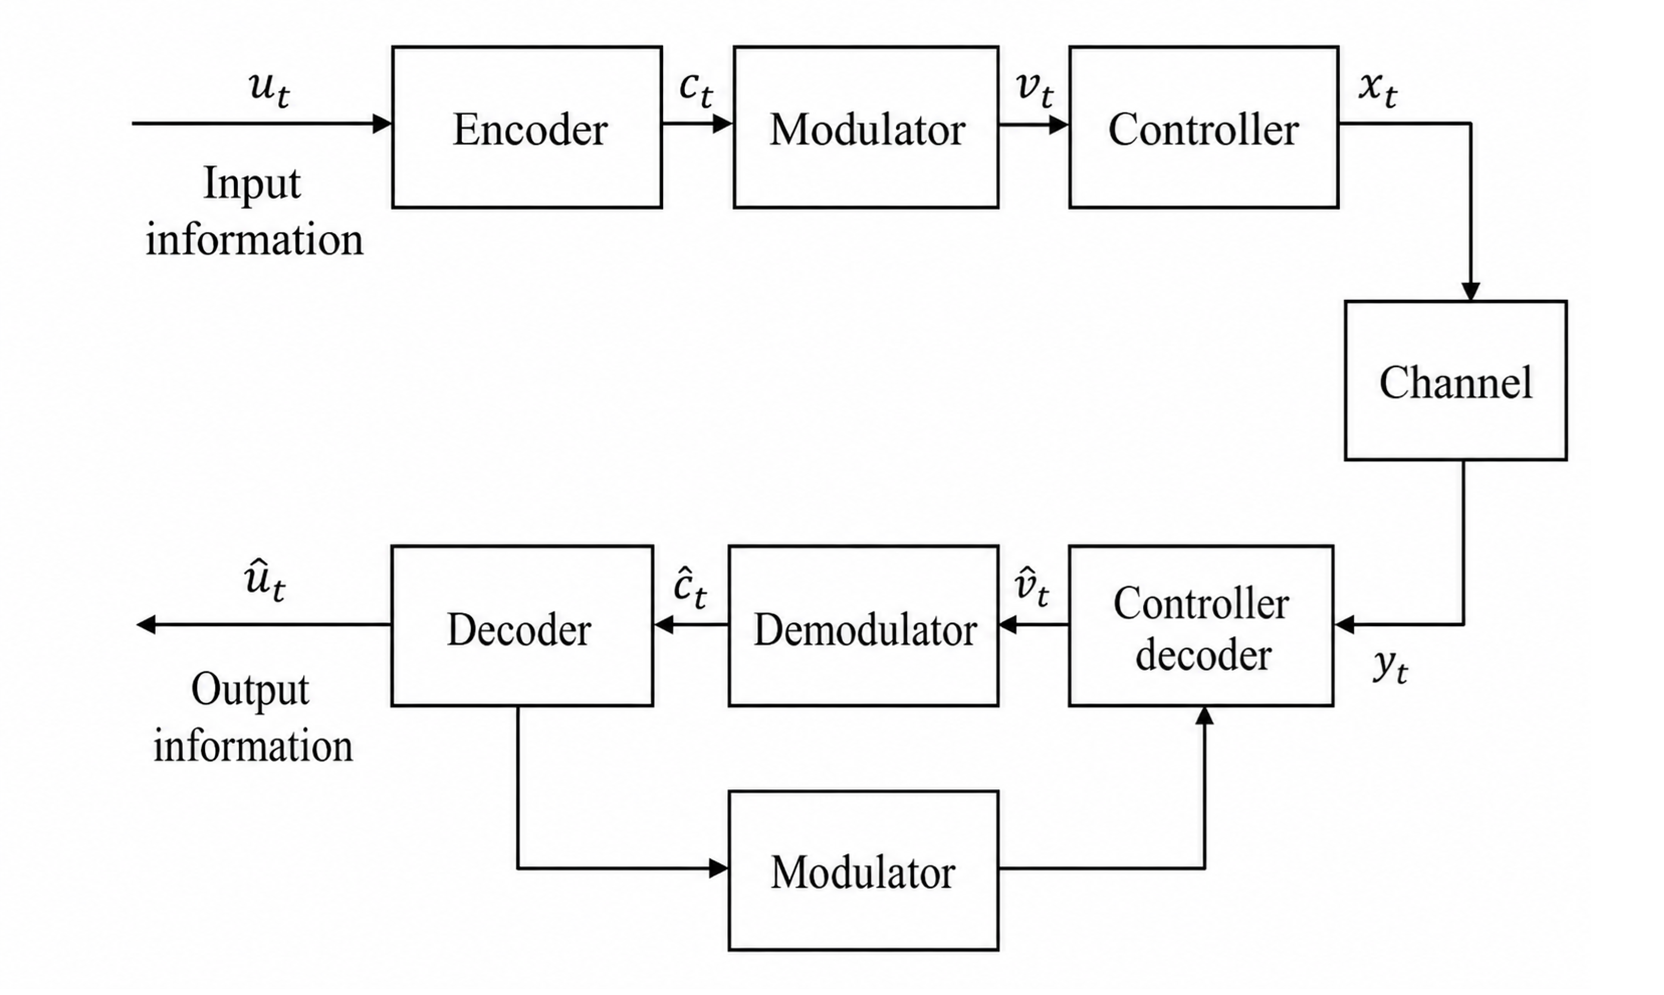
\includegraphics[width=0.96\textwidth]{bibcmid_block_diagram.png}
\caption{BIBCM-ID transmitter, interleaver, channel, and iterative receiver structure.}
\label{fig:bicmid_block}
\end{figure}

Figure~\ref{fig:bicmid_block} shows the coded-modulation chain considered in this thesis. At the transmitter, an information vector is first encoded by a channel code, then permuted by an interleaver, grouped into modulation labels, and converted into channel symbols by the Modulation block. At the receiver, the soft Demodulation block computes bit-level reliability metrics, the deinterleaver restores the code-bit order, and the SISO channel decoder returns extrinsic information through the interleaver to refine the next Demodulation~step.

\begin{equation}
\mathbf{u}_t=\left[u_t^1,u_t^2,\ldots,u_t^k\right]
\xrightarrow{\mathrm{encoder}}
\mathbf{c}_t=\left[c_t^1,c_t^2,\ldots,c_t^n\right].
\end{equation}
The code rate is $R_c=k/n$. Unlike symbol-interleaved coded-modulation structures, BICM-ID and BIBCM-ID interleave coded bits before mapping. The block/bit interleaver of length $N_p$ produces a permuted sequence that can be partitioned into groups of $m=\log_2M$ bits:

\begin{equation}
\mathbf{v}_t=\left[v_t^1,v_t^2,\ldots,v_t^m\right], \qquad t=1,2,\ldots,\frac{N_p}{M}.
\end{equation}
Each bit group is mapped to one point of the signal set $\mathcal{X}$ by the following labeling function:

\begin{equation}
x_t=\mu(\mathbf{v}_t), \qquad x_t\in\mathcal{X}, \qquad |\mathcal{X}|=M.
\end{equation}
For $M$-PSK, the signal set may be written as $x_\ell=e^{j2\pi \ell/M}$, $\ell=0,1,\ldots,M-1$. For square $M$-QAM, a standard constellation can be expressed by

\begin{equation}
\mathcal{X}=\left\{A+jB \mid A,B\in\{\pm1,\pm3,\ldots,\pm(\sqrt{M}-1)\}\right\},
\end{equation}
with a suitable normalization when average symbol energy must be fixed.

After transmission through a flat-fading channel with additive white Gaussian noise, the received symbol can be modeled as

\begin{equation}
y_t=h_t\sqrt{E_s}x_t+n_t,
\end{equation}
where $h_t$ is the channel coefficient, $E_s$ is the symbol energy, and $n_t$ is AWGN with one-sided noise power spectral density $N_0$. Under an AWGN-only channel $h_t=1$, whereas under flat Rayleigh fading $h_t$ is random and the receiver is usually assumed to have channel-state information (CSI) for coherent soft demodulation.

\subsection{Soft Demodulation and Iterative Decoding}
\begin{figure}[H]
\centering
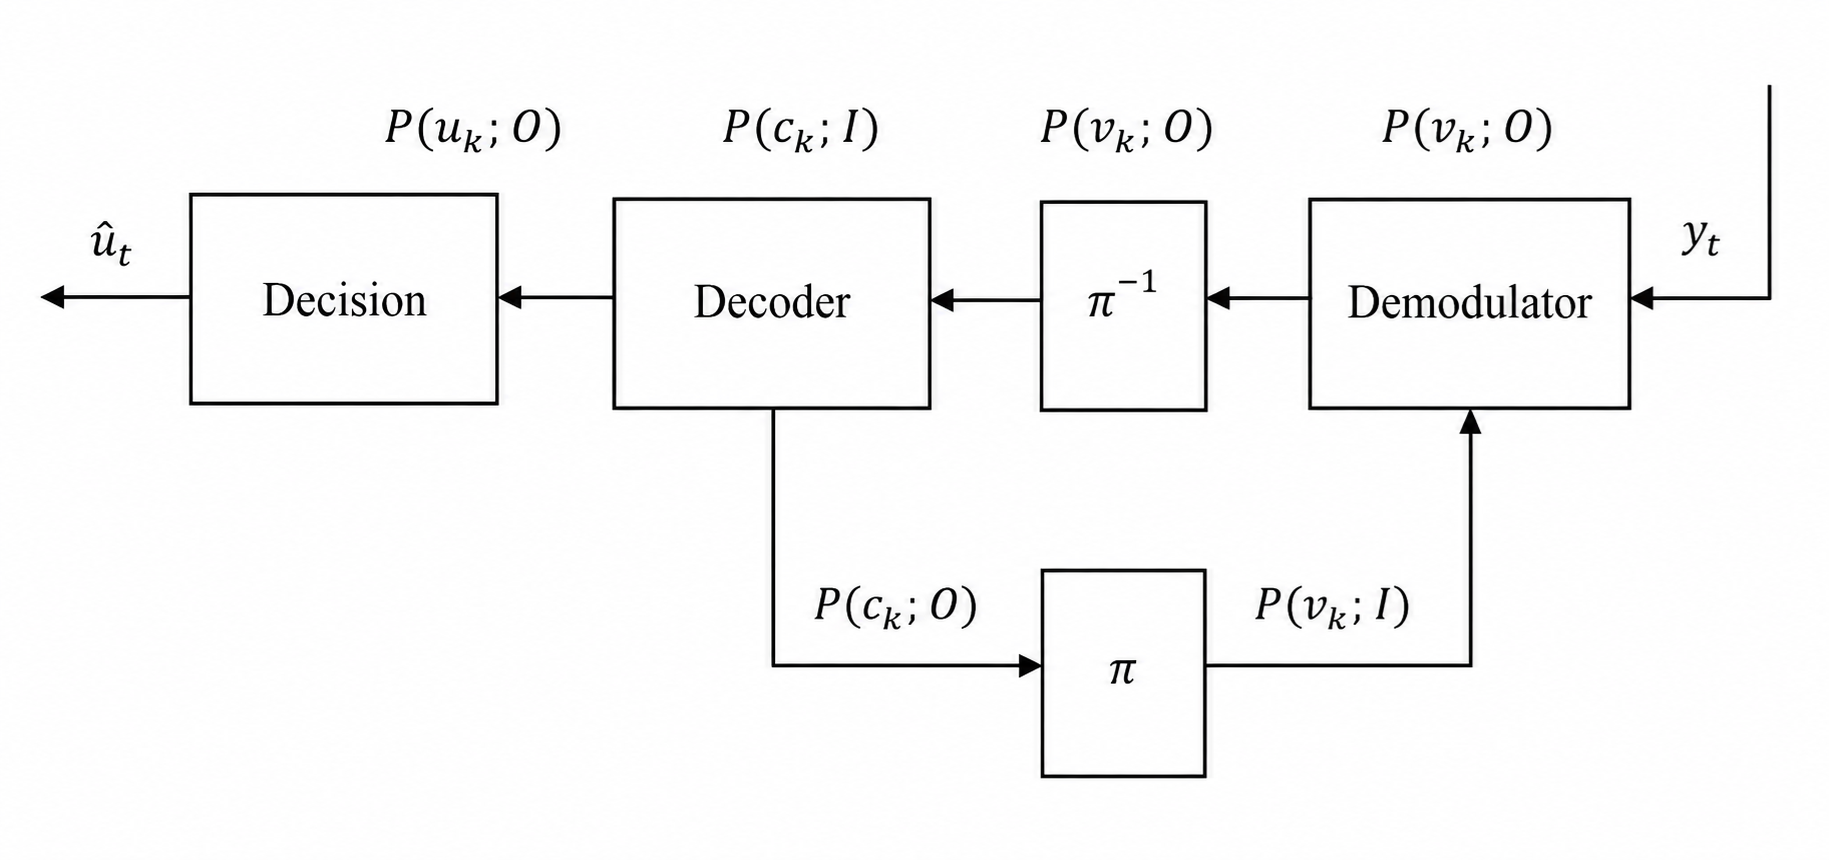
\includegraphics[width=0.88\textwidth]{bibcmid_soft_iteration.png}
\caption{Soft-information exchange between Demodulation and channel decoding in BIBCM-ID.}
\label{fig:bicmid_soft_iteration}
\end{figure}

The receiver in Figure~\ref{fig:bicmid_soft_iteration} follows a soft-input/soft-output (SISO) principle. The soft demodulator computes bit-wise reliability values from the received symbol and channel estimate. Let $\mathcal{X}_b^k$ denote the subset of constellation points whose $k$-th label bit is equal to $b\in\{0,1\}$. A posteriori bit metrics can be written as

\begin{equation}
\lambda(v_k=b)=\log\sum_{x_i\in\mathcal{X}_b^k}\Pr(x_i\mid y,h).
\end{equation}
Using Bayes' rule,

\begin{equation}
\Pr(x_i\mid y,h)=\frac{p(y\mid x_i,h)\Pr(x_i)}{p(y\mid h)},
\qquad
p(y\mid h)=\sum_{i=1}^{M}p(y\mid x_i,h)\Pr(x_i).
\end{equation}
If all transmitted symbols are equally likely, the prior $\Pr(x_i)$ is uniform and the bit metric can be evaluated from the likelihood term alone:

\begin{equation}
\lambda(v_k=b)\sim\log\sum_{x_i\in\mathcal{X}_b^k}p(y\mid x_i,h).
\end{equation}
The corresponding log-likelihood ratio is

\begin{equation}
L(v_k)=\lambda(v_k=1)-\lambda(v_k=0).
\end{equation}
Throughout the thesis, unless otherwise stated, the LLR convention is
\begin{equation*}
L(b|y)=\log\frac{P(b=1|y)}{P(b=0|y)}.
\end{equation*}
A positive LLR therefore favors bit value one, and a negative LLR favors bit value zero. Some references use the opposite sign convention; in such cases the Demodulator output or the hard-decision rule must be sign-adjusted before comparison. These values are deinterleaved and passed to the SISO channel decoder. The decoder computes updated a posteriori and extrinsic information. The extrinsic component is then interleaved and returned as a priori information to the Demodulator. This iterative exchange is the central distinction between BICM and BICM-ID; in BIBCM-ID, the block-interleaving structure further controls the relation between code-bit positions and Modulation-bit positions.

\subsection{Channel Coding}
Channel coding adds structured redundancy so that the receiver can correct errors in noisy and fading channels. In the reference BICM-ID model, convolutional and concatenated codes are discussed as representative channel codes. In this thesis, the channel-coding component is connected to LDPC decoding because the research scope focuses on ANN-assisted LDPC message updates. The LDPC decoder still plays the same system role: it consumes deinterleaved soft information and returns refined reliability information to support the next demodulation iteration.

The check-node update in the Sum-Product Algorithm is accurate but computationally expensive. Simplified methods such as Min-Sum reduce complexity at the cost of performance. This trade-off motivates a neural approximation of the check-node update. The ANN can be trained to reproduce SPA behavior or to modify unreliable messages, while the LDPC graph structure remains intact.

\subsection{Interleaving}
The interleaver permutes coded bits before modulation. This block reduces correlation, spreads burst errors, and changes the relation between code bits and modulation bit positions. In BIBCM-ID, the block interleaver is particularly relevant because extrinsic information should be as independent as possible between demodulator and decoder iterations.

Interleaver design has been studied extensively in recent years. Algebraic interleavers, S-random interleavers, protograph-aware interleavers, and hardware-oriented contention-free interleavers have been proposed to improve convergence, reduce adverse low-weight patterns, and support parallel processing. For this reason, the thesis does not claim novelty in interleaver construction. It acknowledges the interleaver as a key component and focuses on modulation and channel coding.

\section{Soft-Information Processing in BIBCM-ID}
\section{Detailed Soft-Information Model of BIBCM-ID}
The central technical object in BIBCM-ID is the reliability message attached to each coded bit. A conventional receiver can be described as a sequence of hard decisions, but such a description hides the main advantage of iterative coded modulation. In BIBCM-ID, the Demodulation block and the channel decoder exchange soft information. The channel decoder does not only decide whether a bit is zero or one; it evaluates how reliable that decision is. The Demodulation block does not only choose the nearest constellation point; it evaluates the probability of each label bit after observing a noisy channel sample. This distinction is essential because iterative processing can only improve the receiver when the exchanged soft information carries probabilistic meaning.

Let $\mathbf{b}_t=[b_{t,1},\ldots,b_{t,m}]$ denote the bit label associated with a transmitted symbol at time $t$, where $m=\log_2 M$ for an $M$-ary constellation. The Modulation function maps this label to a complex symbol
\begin{equation}
  x_t=\mu(\mathbf{b}_t), \qquad \mu:\{0,1\}^{m}\rightarrow\mathcal{X}.
\end{equation}
For coherent reception over a flat-fading channel, the observation is
\begin{equation}
  y_t=h_t x_t+w_t,
\end{equation}
where $h_t$ is the channel coefficient and $w_t\sim\mathcal{CN}(0,N_0)$ is complex Gaussian noise. The likelihood used by the soft Demodulation block is then
\begin{equation}
  p(y_t|x,h_t)=\frac{1}{\pi N_0}\exp\left(-\frac{|y_t-h_t x|^2}{N_0}\right).
\end{equation}
This likelihood is the bridge between the analog received sample and the digital LDPC decoder. If the likelihood is accurately modeled, the resulting LLR values are statistically meaningful. If the likelihood is mismatched, the decoder receives biased reliability messages even when the hard-decision symbol error rate appears acceptable.

For the $k$-th bit of a symbol label, define the two subsets
\begin{equation}
  \mathcal{X}_{k}^{(b)}=\{x\in\mathcal{X}: b_k(x)=b\}, \qquad b\in\{0,1\}.
\end{equation}
When no a priori information is available from the decoder, the demodulator LLR can be written as
\begin{equation}
  L_{\mathrm{dem}}(b_k|y_t)
  =\log\frac{\sum_{x\in\mathcal{X}_{k}^{(1)}}p(y_t|x,h_t)}
  {\sum_{x\in\mathcal{X}_{k}^{(0)}}p(y_t|x,h_t)}.
\end{equation}
At later iterations, however, the Demodulation block receives a priori bit information from the decoder. In that case, the symbol prior is no longer uniform. If the a priori LLR of label bit $b_i$ is $L_A(b_i)$, the prior probability of a candidate label can be expressed as
\begin{equation}
  P_A(\mathbf{b}(x))=
  \prod_{i=1}^{m}
  \frac{\exp(b_i(x)L_A(b_i))}
  {1+\exp(L_A(b_i))}.
\end{equation}
The updated a posteriori Demodulation LLR becomes
\begin{equation}
  L_{\mathrm{APP}}(b_k|y_t)
  =
  \log
  \frac{\sum_{x\in\mathcal{X}_{k}^{(1)}}p(y_t|x,h_t)
  \prod_{i\ne k} P_A(b_i(x))}
  {\sum_{x\in\mathcal{X}_{k}^{(0)}}p(y_t|x,h_t)
  \prod_{i\ne k} P_A(b_i(x))}.
\end{equation}
The extrinsic output of the Demodulation block is obtained by removing the a priori contribution of the same bit:
\begin{equation}
  L_E^{\mathrm{dem}}(b_k)=L_{\mathrm{APP}}(b_k|y_t)-L_A(b_k).
\end{equation}
This subtraction is not a cosmetic detail. It prevents the same evidence from being counted repeatedly in the iterative loop. If the receiver repeatedly feeds back a message that includes its own previous information, the iterative process can become artificially confident and may converge to a codeword that violates parity constraints.

The computational burden of exact LLR evaluation grows with the constellation size because the demodulator sums over subsets of $\mathcal{X}$. For large $M$, the max-log approximation is often used:
\begin{equation}
  L_{\mathrm{dem}}(b_k|y_t)
  \approx
  \frac{1}{N_0}
  \left[
  \min_{x\in\mathcal{X}_{k}^{(0)}}|y_t-h_t x|^2
  -
  \min_{x\in\mathcal{X}_{k}^{(1)}}|y_t-h_t x|^2
  \right].
\end{equation}
This expression is attractive because it replaces sums of exponentials by distance comparisons. Nevertheless, the approximation changes the magnitude of LLRs. In a one-shot receiver, a magnitude error may have limited effect if the sign is correct. In an iterative receiver, a magnitude error changes the influence of the message on subsequent decoding iterations. Therefore, LLR scaling, clipping, and calibration are not secondary implementation details; they directly affect BIBCM-ID convergence.

A practical receiver commonly clips LLRs to a finite interval:
\begin{equation}
  \tilde{L}=\mathrm{clip}(L,L_{\min},L_{\max}).
\end{equation}
Clipping protects the decoder from numerical overflow and reduces memory width in fixed-point hardware. However, overly aggressive clipping removes reliability information, while insufficient clipping allows rare overconfident values to dominate the decoder. This issue is closely related to the ANN-assisted LDPC part of the thesis. A neural check-node update can be interpreted as a learned nonlinear transformation of reliability messages; its value depends not only on the final hard decision but also on how it reshapes message magnitudes during iterations.

\section{Role of Labeling, Interleaving, and Iterative Gain}
The mapping between bit labels and constellation points affects the reliability profile of the Demodulation output. In conventional non-iterative BICM, Gray labeling is usually preferred because adjacent constellation points differ in one bit, reducing the number of bit errors caused by a symbol error. In BICM-ID and BIBCM-ID, the best labeling may differ because the Demodulation block can exploit a priori information from the channel decoder. Set-partitioning labels, anti-Gray labels, and other mappings can provide stronger iterative gain under certain conditions because they create different extrinsic-information transfer characteristics.

This point clarifies why Modulation is relevant even when the thesis title emphasizes LDPC decoding. The LDPC decoder receives LLR values whose distribution is determined partly by the constellation geometry and labeling rule. A decoder-side improvement cannot fully compensate for a Demodulation block that consistently produces poorly calibrated or weak LLRs. Conversely, a Modulation/Demodulation design that produces more separable and better-calibrated reliability messages can make the LDPC decoder more effective without changing the parity-check matrix.

For a label bit $b_k$, define the conditional LLR density $p(L|b_k)$. A good Demodulation design should not only shift the mean of this density away from zero; it should also reduce harmful overlap between the densities conditioned on $b_k=0$ and $b_k=1$. The mutual information between a bit and its LLR is often used to summarize this behavior:
\begin{equation}
  I(B;L)=
  \sum_{b\in\{0,1\}}\int p(b,L)
  \log_2\frac{p(b,L)}{p(b)p(L)}\,dL.
\end{equation}
In EXIT-chart analysis, the Demodulation block and the channel decoder are viewed as two components that transform input mutual information into output mutual information. Although this thesis does not construct full EXIT charts, the underlying idea is important: iterative gain appears when the transfer curve of the Demodulation block and the transfer curve of the decoder leave an open convergence tunnel. If the Demodulation output saturates too early or the decoder cannot exploit the a priori information, additional iterations provide little benefit.

The block interleaver changes the statistical relationship between neighboring coded bits and neighboring modulation positions. Suppose the encoder output is $\mathbf{c}=[c_1,\ldots,c_N]$ and the interleaver is a permutation $\pi$ on $\{1,\ldots,N\}$. The interleaved sequence is
\begin{equation}
  v_i=c_{\pi(i)}.
\end{equation}
For an ideal random interleaver, bits that are nearby in the code graph are likely to be separated across different symbol positions. A block interleaver imposes a more structured permutation, which can be beneficial for implementation and memory access. The design objective is to reduce harmful correlation while supporting practical hardware constraints such as parallel read/write access and deterministic addressing.

From the decoder viewpoint, interleaving also affects error events. If several unreliable channel observations are mapped to code bits that participate in closely related parity checks, the decoder may see a concentrated reliability deficit. A good interleaver spreads such unreliable bits so that parity constraints can compensate for them. This is why interleaver design has a strong literature of its own. The thesis treats it as a mature and essential part of the BIBCM-ID framework, while focusing the technical contribution on the decoder-side ANN approximation and the supporting Modulation/Demodulation study.

The BIBCM-ID iteration can be summarized by two coupled transformations:
\begin{equation}
  \mathbf{L}_{E,\mathrm{dem}}^{(t)}
  =
  \mathcal{M}\left(\mathbf{y},\Pi\mathbf{L}_{E,\mathrm{dec}}^{(t-1)}\right),
\end{equation}
\begin{equation}
  \mathbf{L}_{E,\mathrm{dec}}^{(t)}
  =
  \mathcal{D}\left(\Pi^{-1}\mathbf{L}_{E,\mathrm{dem}}^{(t)}\right).
\end{equation}
Here $\mathcal{M}$ denotes soft Demodulation and $\mathcal{D}$ denotes channel decoding. The LDPC decoder is therefore not an isolated block. It is one component in a feedback loop whose behavior depends on message quality, message independence, and message scaling. This observation is used throughout the thesis to justify why the ANN-assisted LDPC study should be evaluated in terms of both BER and message-processing complexity.

\section{Practical Receiver Issues Relevant to the Thesis}
Several practical receiver issues are important for interpreting the simulation results. First, the LLR sign convention must be used consistently. This thesis uses
\begin{equation}
  L(b|y)=\log\frac{P(b=1|y)}{P(b=0|y)},
\end{equation}
so a positive LLR favors bit value one. Some references define the opposite sign. A sign mismatch between Demodulation and decoding would make the decoder reinforce the wrong hypothesis. Therefore, whenever a different BPSK mapping or reference convention is used, the sign must be converted before the hard decision and before the LLR is passed to the LDPC decoder.

Second, SNR normalization affects both Demodulation and decoding. For coded modulation, the relationship between symbol energy and bit energy is
\begin{equation}
  E_b=\frac{E_s}{R_c\log_2 M},
\end{equation}
so that
\begin{equation}
  \left(\frac{E_b}{N_0}\right)_{\mathrm{dB}}
  =
  \left(\frac{E_s}{N_0}\right)_{\mathrm{dB}}
  -
  10\log_{10}(R_c\log_2 M).
\end{equation}
If this conversion is not handled carefully, curves for different coding rates or modulation orders may be compared unfairly. This is one reason why the thesis avoids making broad superiority claims from a single BER curve.

Third, fixed-point implementation changes message behavior. A floating-point simulation can represent very small probability differences and very large LLR magnitudes. A hardware decoder normally uses quantized message values:
\begin{equation}
  L_Q=Q_{\Delta,L_{\max}}(L),
\end{equation}
where $Q_{\Delta,L_{\max}}(\cdot)$ denotes a quantizer with step size $\Delta$ and clipping limit $L_{\max}$. Quantization can degrade SPA more than Min-Sum in some settings because precise nonlinear corrections are lost. This observation strengthens the motivation for a compact ANN approximation: a learned function can be trained or fine-tuned under quantization constraints instead of being derived only for ideal real-valued arithmetic.

Fourth, the number of iterations is part of the system design. More iterations usually improve BER up to a point, but they increase latency and power consumption. Let $I_{\max}$ be the maximum number of decoding iterations and $E$ be the number of edges in the Tanner graph. A message-passing decoder has a computational load that scales approximately with $I_{\max}E$. If an ANN check-node update reduces the cost per edge but requires more iterations to converge, the net benefit may be small. Therefore, the thesis interprets ANN assistance through convergence behavior and the computational cost of each update.

Finally, the receiver must remain robust to model mismatch. The Demodulation formula derived for AWGN does not fully describe PA nonlinearity, CFO, or multipath fading. Similarly, an ANN trained on one distribution of messages may not generalize to another distribution. The most credible engineering interpretation is therefore not that neural networks automatically outperform classical methods, but that they provide trainable approximations for specific nonlinear or mismatched operations when the training and validation conditions are carefully defined.


\section{Machine Learning and Deep Learning Foundations}
Machine learning is a family of computational methods in which a model improves its behavior from data rather than from a completely hand-written rule set \cite{bishop2006}. In communication engineering, this viewpoint is useful because many receiver functions are derived from idealized mathematical assumptions. A demodulator may assume additive Gaussian noise, a decoder may assume independent messages, and a synchronizer may assume a known impairment model. Practical wireless channels often violate these assumptions. Machine learning provides a way to learn corrections, approximations, or decision rules from measured or simulated examples while still retaining the structure of the communication system.

A supervised learning problem can be written as the minimization of an empirical risk:
\begin{equation}
\label{eq:ml_empirical_risk}
\theta^\star=\arg\min_{\theta}\frac{1}{N}\sum_{n=1}^{N}
\ell\!\left(f_{\theta}(\mathbf{x}_n),\mathbf{t}_n\right)
+\lambda\Omega(\theta),
\end{equation}
where $\mathbf{x}_n$ is the input sample, $\mathbf{t}_n$ is the desired target, $f_{\theta}(\cdot)$ is the model, $\ell(\cdot)$ is the loss function, and $\Omega(\theta)$ is a regularization term. In a physical-layer receiver, $\mathbf{x}_n$ may be a vector of received samples, LLRs, channel estimates, or Tanner-graph messages. The target $\mathbf{t}_n$ may be a transmitted bit, an SPA message, a channel state, or a calibrated probability. Equation~\eqref{eq:ml_empirical_risk} is general, but the engineering meaning of the target is critical. A model trained for hard classification is not automatically suitable for iterative decoding, because BIBCM-ID requires reliable soft information rather than only final bit decisions.

Deep learning is a subset of machine learning based on multi-layer parameterized models \cite{lecun2015,goodfellow2016}. A feed-forward neural network layer can be expressed as
\begin{equation}
\label{eq:nn_layer_ch1}
\mathbf{z}^{(\ell)}=\sigma\!\left(\mathbf{W}^{(\ell)}\mathbf{z}^{(\ell-1)}+\mathbf{b}^{(\ell)}\right),
\end{equation}
where $\mathbf{W}^{(\ell)}$ and $\mathbf{b}^{(\ell)}$ are trainable parameters and $\sigma(\cdot)$ is a nonlinear activation function. Multiple layers allow the network to represent nonlinear mappings that would otherwise require complicated analytical approximations. This property is relevant for LDPC decoding because the SPA check-node update contains nonlinear operations, and it is relevant for learned Modulation because the optimal signal geometry under PA nonlinearity, CFO, fading, and noise is not always captured by a fixed QAM constellation.

Training is usually performed by gradient-based optimization. For a mini-batch $\mathcal{B}$, a generic update is
\begin{equation}
\label{eq:gradient_update_ch1}
\theta_{r+1}=\theta_r-\eta\nabla_{\theta}
\left[\frac{1}{|\mathcal{B}|}\sum_{n\in\mathcal{B}}
\ell\!\left(f_{\theta_r}(\mathbf{x}_n),\mathbf{t}_n\right)\right],
\end{equation}
where $\eta$ is the learning rate. Modern optimizers such as Adam modify the effective step size using first- and second-order moment estimates, but the principle remains the same: the parameters are adjusted so that model outputs become closer to the targets. For communication systems, the training distribution must be treated carefully. If the model is trained only at one SNR, one channel realization, or one hardware impairment level, it may not generalize to the operating range of a real receiver.

\begin{table}[H]
\centering
\caption{Learning paradigms relevant to communication receiver design.}
\label{tab:learning_paradigms}
\begin{tabularx}{\textwidth}{>{\raggedright\arraybackslash}p{0.25\textwidth}>{\raggedright\arraybackslash}p{0.33\textwidth}>{\raggedright\arraybackslash}X}
\toprule
Paradigm & Typical target & Communication example\\
\midrule
Supervised learning & Known labels or reference outputs & Bit classification, SPA-message imitation, channel estimation from pilots\\
Unsupervised learning & Structure in unlabeled data & Clustering received constellations, blind impairment detection\\
Reinforcement learning & Long-term reward from interaction & Adaptive resource allocation, link adaptation, scheduling\\
Model-driven learning & Parameters embedded in known algorithms & Neural BP, learned Min-Sum correction, trainable Demodulation metrics\\
\bottomrule
\end{tabularx}
\end{table}

Table~\ref{tab:learning_paradigms} summarizes several learning paradigms that appear in communication research. The most relevant paradigm for this thesis is model-driven learning. Instead of replacing the receiver by a fully black-box network, model-driven learning keeps a known algorithmic structure and introduces trainable components at selected points. This is the reason the LDPC part of the thesis focuses on a local neural approximation of the check-node update, and the Modulation part focuses on a learned signal representation under specified channel impairments.

\section{Deep Learning Applications in Telecommunications}
Deep learning has been investigated in many parts of modern telecommunications, from the physical layer to network management \cite{oshea2017,cammerer2020}. At the physical layer, the main motivation is the difficulty of modeling all impairments exactly. Real receivers face nonlinear power amplifiers, oscillator mismatch, imperfect channel estimation, quantized front-end samples, phase noise, interference, and fading. Classical signal processing remains essential because it gives interpretable models and stability guarantees, but learning-based methods can complement it when the analytical model is incomplete or too costly for direct implementation.

In channel estimation, neural networks can learn mappings from pilot observations to channel coefficients. This is useful when the channel has spatial, temporal, or frequency-domain structure that is not fully exploited by a simple least-squares estimator. In signal detection, neural receivers can learn decision boundaries in nonlinear or mismatched channels. In synchronization, sequence models can exploit temporal dependencies caused by CFO or phase noise. In channel decoding, neural belief propagation, trainable Min-Sum variants, and local message-update networks aim to improve or simplify iterative decoding. In resource allocation, reinforcement learning can adapt scheduling, power control, and beam selection when the environment changes over time.

\begin{table}[H]
\centering
\caption{Deep-learning applications related to telecommunications systems.}
\label{tab:dl_telecom_applications}
\begin{tabularx}{\textwidth}{>{\raggedright\arraybackslash}p{0.24\textwidth}>{\raggedright\arraybackslash}p{0.34\textwidth}>{\raggedright\arraybackslash}X}
\toprule
Area & Learning task & Relevance to this thesis\\
\midrule
Modulation and Demodulation & Learned constellation, detector, or LLR estimator & Directly related to the AutoEncoder Modulation study\\
Channel coding & Neural BP, learned Min-Sum, decoder approximation & Directly related to ANN-assisted LDPC decoding\\
Channel estimation & Pilot-based or data-aided estimation & Affects the likelihood used for soft Demodulation\\
Synchronization & CFO and phase-noise tracking & Motivates sequence-based neural Demodulation\\
Hardware impairment mitigation & PA, IQ imbalance, quantization correction & Supports the non-ideal channel analysis\\
Network control & Link adaptation, scheduling, beam management & Related at system level but outside the thesis scope\\
\bottomrule
\end{tabularx}
\end{table}

Table~\ref{tab:dl_telecom_applications} places the thesis within the wider telecommunications literature. The table also clarifies the boundary of the research. The thesis does not study network-layer optimization, scheduling, or beam management. It concentrates on two physical-layer interfaces: the Modulation/Demodulation interface that produces bit-level reliability and the LDPC decoder that processes reliability through parity constraints.

For BIBCM-ID, the most important point is that learning should respect the soft-information interface. A neural classifier that outputs only hard bits is not sufficient for iterative decoding. The receiver needs probability-like outputs or LLR-like values that can be exchanged between the Demodulator and the LDPC decoder. If a neural model produces overconfident probabilities, the iterative loop can become unstable or converge to a wrong codeword. Therefore, calibration is a central requirement. One common form of calibration introduces a temperature parameter $T$:
\begin{equation}
\label{eq:temperature_scaling_ch1}
\hat{p}_T(c|\mathbf{x})=
\frac{\exp(a_c/T)}
{\sum_{c'}\exp(a_{c'}/T)},
\end{equation}
where $a_c$ is the logit for class $c$. Larger $T$ softens the distribution, while smaller $T$ makes it more confident. For learned Demodulation, such calibration affects the LLR magnitude delivered to the LDPC decoder. This connection explains why Chapter~2 studies learned Modulation/Demodulation before Chapter~3 analyzes the ANN-assisted LDPC decoder in detail.

The use of deep learning in this thesis is therefore deliberately conservative. Classical communication blocks define the signal chain, equations, and evaluation metrics. Neural networks are introduced only where they have a clear technical role: learning a channel-aware signal representation, approximating nonlinear message updates, and improving or regulating reliability values. This hybrid position is more suitable for an engineering thesis than a purely black-box interpretation, because it preserves interpretability and allows fair comparison with SPA, Min-Sum, QAM, and conventional likelihood-based Demodulation.


\section{Related Work on BIBCM-ID and Neural Receivers}
The technical background of this thesis is built on three research lines. The first line is LDPC coding and iterative message-passing decoding. Gallager's original LDPC construction, Tanner-graph representation, factor-graph inference, SPA decoding, and Min-Sum variants provide the mathematical basis for the ANN-assisted decoder studied in Chapter 3 \cite{gallager1962,tanner1981,kschischang2001,hu2001spa,chen2002}. This literature is important because the neural model in this thesis is not a replacement for coding theory; it is a compact approximation of a well-defined check-node operation.

The second line is BICM-ID/BIBCM-ID. Bit-interleaved coded modulation combines channel coding, bit interleaving, and high-order Modulation \cite{zehavi1992,caire1998,li1997,li1998}. Iterative Demodulation and decoding improve performance by exchanging extrinsic information between the Demodulation block and the channel decoder. In this setting, the quality of LLR values is as important as the final hard decision, because unreliable soft information can slow convergence or strengthen wrong decisions.

The third line is deep learning for physical-layer communication. Neural belief-propagation methods, learned Min-Sum corrections, and compact neural decoders show that model-driven learning can improve or simplify iterative decoding \cite{nachmani2016,nachmani2018,lugosch2017,kuck2020,wang2022}. AutoEncoder-based communication studies show that learned Modulation and Demodulation can adapt to channel impairments such as PA nonlinearity, CFO, fading, and noise \cite{oshea2017,dorner2018,aoudia2019,rapp1991,saleh1981}. In this thesis, these works are used to support a hybrid viewpoint: the established BIBCM-ID processing chain is retained, while neural networks are studied as tools for nonlinear approximation, reliability control, and channel-aware signal representation.

Across these research lines, the common engineering criterion is not only BER. A useful method should also preserve soft-information meaning, control computational complexity, avoid overconfident unreliable messages, and remain robust when the actual channel differs from the training or design model. This criterion motivates the detailed discussion of LLR reliability in this section.

A central internal variable of a BIBCM-ID receiver is not the hard bit decision but the reliability attached to each bit. This reliability is usually represented by an LLR. A positive LLR favors one bit value, a negative LLR favors the other, and the magnitude indicates confidence. In an iterative receiver, the magnitude is as important as the sign because it determines how strongly later blocks trust the message.

If the channel model is correct, LLR computation has a clear probabilistic meaning. If the channel model is mismatched, the same formula may produce overconfident or underconfident values. For example, a demodulator that ignores PA compression may treat a distorted outer constellation point as if it were produced by Gaussian noise only. The resulting LLR may be biased. When this biased information is passed to the LDPC decoder, the decoder may reinforce an incorrect belief.

This reliability problem motivates both research directions of the thesis. In channel decoding, the ANN check-node update attempts to improve or approximate the reliability message generated inside the LDPC graph. In modulation, the autoencoder attempts to create a signal representation that is easier to detect reliably under non-ideal channels. Both directions are therefore connected by the same underlying question: how can the system produce more useful soft information?

The interleaver also affects soft-information reliability, but in a different way. It does not compute reliability; it changes the dependence pattern between bits. A well-designed interleaver can reduce adverse correlation and distribute unreliable bits more evenly. Nevertheless, because the present thesis does not design a new interleaver, the reliability-improvement effort is directed toward modulation and decoding.

A technically consistent thesis separates message accuracy from final BER. BER is the final measure, but it does not explain why a method works. A neural demodulator or neural decoder may reduce BER because it improves reliability calibration, because it regularizes overconfident messages, because it changes the effective decision boundary, or because it overfits to a tested condition. The analysis in this thesis interprets BER together with model structure and channel assumptions.

The distinction between intrinsic and extrinsic information is also important. The demodulator starts from received samples and may use a priori information from the decoder. The decoder receives demodulator output and returns extrinsic information that should not simply repeat the same evidence. If the same information is counted multiple times, the iterative loop can become overconfident. This issue is closely related to short cycles in LDPC graphs and to interleaver design in BIBCM-ID.

Deep learning can help with reliability when the training objective reflects reliability. If a network is trained only for hard classification, it may output probabilities that are not calibrated. For BIBCM-ID, a soft-output network can be trained or post-processed so that its output magnitude has meaning. This requirement is one reason why AutoEncoder Modulation is discussed as supporting evidence for the Modulation/Demodulation interface rather than as the main LDPC-decoder contribution.

A practical research path is to begin with well-defined processing functions and calibrated interfaces. The ANN-LDPC work is already aligned with message passing because it outputs check-node messages inside the LDPC decoder. The AutoEncoder Modulation work is therefore used as supporting evidence for the Modulation/Demodulation side of the soft-information interface, especially under channel impairments that can bias conventional LLR~computation.

\begin{equation}
\label{eq:llr_definition_ch1}
L(b_k|y)=\ln\frac{P(b_k=1|y)}{P(b_k=0|y)}.
\end{equation}
Equation~\eqref{eq:llr_definition_ch1} defines the log-likelihood ratio of bit $b_k$ given the received observation $y$. The sign of the LLR indicates the more likely bit value, while the magnitude represents confidence. In iterative decoding, this magnitude must be interpreted carefully because overconfident wrong information can be more detrimental than weak information.

\begin{equation}
\label{eq:extrinsic_definition_ch1}
L_{\mathrm{E}}(b_k)=L_{\mathrm{APP}}(b_k)-L_{\mathrm{A}}(b_k)-L_{\mathrm{ch}}(b_k).
\end{equation}
Equation~\eqref{eq:extrinsic_definition_ch1} expresses the extrinsic-information principle. A receiver block should pass new information to the next block, not simply return the same evidence it received. This principle is one reason interleaving is important in BIBCM-ID: it helps reduce statistical dependence between exchanged~messages.

\begin{equation}
\label{eq:decoder_iteration_ch1}
\mathbf{L}^{(t)}_{\mathrm{dec}}=
\mathcal{D}\!\left(\mathbf{L}_{\mathrm{ch}},\Pi^{-1}\mathbf{L}^{(t)}_{\mathrm{dem}}\right).
\end{equation}
Equation~\eqref{eq:decoder_iteration_ch1} gives a compact view of one decoding iteration. The channel decoder $\mathcal{D}$ receives channel reliability and deinterleaved demodulation messages at iteration $t$. Its output then becomes new extrinsic information for the next demodulation step.

\begin{equation}
\label{eq:demod_iteration_ch1}
\mathbf{L}^{(t+1)}_{\mathrm{dem}}=
\mathcal{G}\!\left(\mathbf{y},\Pi\mathbf{L}^{(t)}_{\mathrm{dec}}\right).
\end{equation}
Equation~\eqref{eq:demod_iteration_ch1} shows the feedback direction from the channel decoder to the Demodulation block. The soft-Demodulation operator $\mathcal{G}$ uses the received observation $\mathbf{y}$ and interleaved a priori information to produce updated bit~reliabilities.

\begin{equation}
\label{eq:ber_definition_ch1}
\mathrm{BER}=\frac{N_{\mathrm{err}}}{N_{\mathrm{bit}}}.
\end{equation}
Equation~\eqref{eq:ber_definition_ch1} defines the BER used throughout the thesis. Although BER is the final performance metric, it should be interpreted together with the number of simulated bits and the channel scenario.

\section{Research Scope and Contributions}
The preceding sections show that BIBCM-ID should be analyzed as a soft-information processing system rather than only as a concatenation of independent transmitter and receiver blocks. This thesis therefore defines its research scope at the two interfaces where the available results are technically strongest and most relevant: the LDPC decoder message-update mechanism and the Modulation/Demodulation side that produces soft reliability information for the decoder.

\begin{itemize}
\item The first scope item is to analyze the BIBCM-ID system and clarify the roles of Modulation, Demodulation, channel coding, and interleaving in the iterative receiver.
\end{itemize}
\begin{itemize}
\item The central contribution is the thesis-level formulation and interpretation of ANN-assisted LDPC decoding, with emphasis on compact neural approximation of the check-node update and reliability-aware message adjustment.
\end{itemize}
\begin{itemize}
\item The supporting contribution is the analysis of AutoEncoder-based Modulation under non-ideal channels, including PA nonlinearity, CFO, fading, and the implications for soft-output Demodulation.
\end{itemize}
\begin{itemize}
\item The thesis positions learned Modulation/Demodulation as a complementary direction that supports the BIBCM-ID soft-information interface, while ANN-assisted LDPC decoding remains the main technical contribution.
\end{itemize}

This scope deliberately avoids presenting the interleaver as a new contribution. Interleaver design is recognized as an important and active research direction, but the present work uses it as part of the BIBCM-ID framework. The research effort is instead directed toward neural processing where the available mathematical model, simulation evidence, and engineering interpretation are sufficiently clear for a master's thesis in telecommunications engineering.

\section{Chapter Conclusion}
This chapter has established the technical foundation and research scope of the thesis. The BIBCM-ID receiver has been described as an iterative coded-modulation structure in which Modulation, Demodulation, interleaving, and channel decoding are connected through soft information rather than through hard decisions alone. This viewpoint is important because the LDPC decoder does not operate on ideal transmitted bits; it operates on LLR values whose sign and magnitude are shaped by the channel, the constellation, the labeling rule, the interleaver, and the Demodulation method.

The discussion has also clarified the role of the three main BIBCM-ID components. Modulation and Demodulation determine the geometry and reliability of the received observations. Channel coding, represented in this thesis by LDPC decoding, provides the parity constraints and message-passing mechanism used to correct errors. The interleaver controls the statistical dependence between coded bits and modulation positions, thereby influencing the effectiveness of iterative exchange. Although interleaver design is an active research topic, the present work does not propose a new interleaver; it treats the interleaver as an essential system component and concentrates on the two processing directions supported by the available research results.

From this foundation, the thesis adopts a controlled deep-learning perspective. Neural networks are not introduced as black-box replacements for the communication system. They are considered where they can approximate nonlinear processing, reshape unreliable soft messages, or adapt signal representation under channel mismatch. This chapter therefore justifies the two following technical directions: ANN-assisted LDPC decoding as the central contribution, and learned Modulation/Demodulation as a supporting study of the soft-information source that feeds the decoder.

The next chapter studies learned Modulation and Demodulation before the thesis turns to the LDPC decoder. This ordering is useful because the decoder receives reliability information produced upstream by the Demodulation block. A clear understanding of learned signal representation and LLR quality therefore provides the context for the ANN-assisted LDPC decoding analysis in Chapter 3.

\chapter[\textbf{DEEP LEARNING FOR MODULATION}]{DEEP LEARNING FOR INTELLIGENT MODULATION}
\section{Why Modulation Is a Learning Target}
Modulation determines how coded bits become physical signals. In an ideal channel, conventional constellations such as 16-QAM are efficient and well understood. In non-ideal channels, however, the constellation observed at the receiver may differ significantly from the transmitted one. PA nonlinearity compresses amplitudes, CFO rotates phases, fading changes gain, and ISI introduces memory.

These impairments are not only visual distortions. They directly affect LLR computation. A demodulator that assumes a clean 16-QAM constellation may assign incorrect reliability to received samples. In iterative decoding, incorrect reliability can reduce convergence or cause error propagation. This makes modulation and demodulation important candidates for learning-based correction.

Autoencoder-based modulation studies the communication link as a trainable system. The transmitter network maps messages to normalized channel symbols. The channel layer adds noise and impairments. The receiver network estimates the transmitted message. This framework allows the signal representation to adapt to the channel used during training.

\begin{equation}
y=hx+n.
\end{equation}
Equation (2.1) is the basic flat-fading channel model. The transmitted symbol x is multiplied by a channel coefficient h and corrupted by additive noise n. More complex impairments such as PA nonlinearity, CFO, and ISI modify this basic relation.

\begin{equation}
L(b_k|y)=\ln\frac{\sum_{s\in\mathcal{S}_{k,1}}\exp(-|y-hs|^2/N_0)}
{\sum_{s\in\mathcal{S}_{k,0}}\exp(-|y-hs|^2/N_0)}.
\end{equation}
Equation (2.2) is the bit-level LLR for a conventional constellation under a Gaussian-noise assumption. S\_k\textasciicircum{}1 and S\_k\textasciicircum{}0 are the subsets of constellation points whose kth bit is 1 or 0. When the actual channel includes nonlinear distortion, this expression may become mismatched.

\begin{equation}
\mathrm{PAPR}=\frac{\max_n |x[n]|^2}{\mathbb{E}\{|x[n]|^2\}}.
\end{equation}
Equation (2.3) defines the peak-to-average power ratio. PAPR is relevant because high-amplitude symbols are more vulnerable to PA nonlinearity.

\begin{equation}
d_{\min}=\min_{i\ne j}\|s_i-s_j\|_2.
\end{equation}
Equation (2.4) defines the minimum Euclidean distance of a constellation. Larger distance usually improves noise robustness, but nonlinear channels can change the effective distances after transmission.

\begin{figure}[H]
\centering
\begin{subfigure}{0.47\textwidth}
\centering
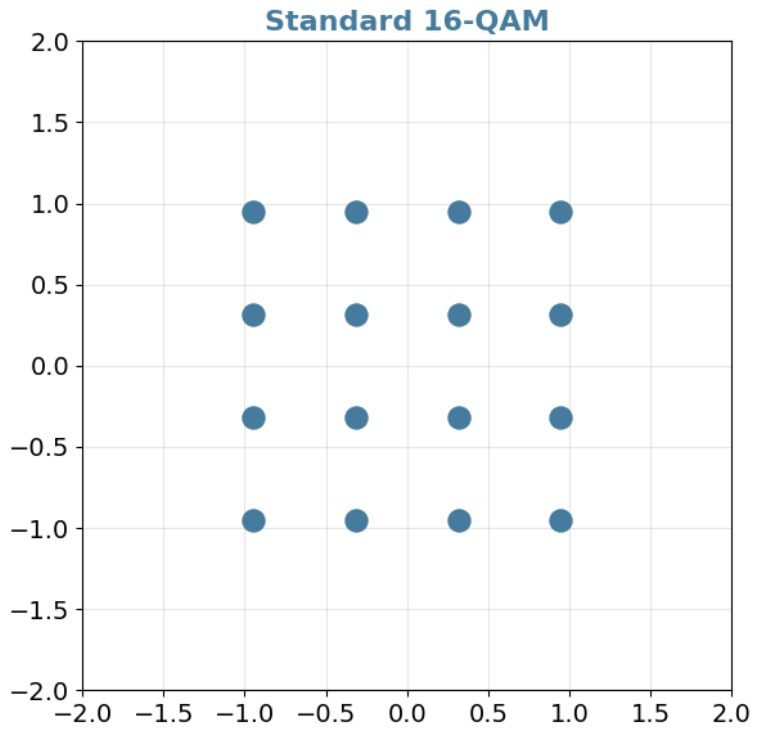
\includegraphics[width=\textwidth]{qam16.png}
\caption{Reference 16-QAM constellation.}
\end{subfigure}\hfill
\begin{subfigure}{0.47\textwidth}
\centering
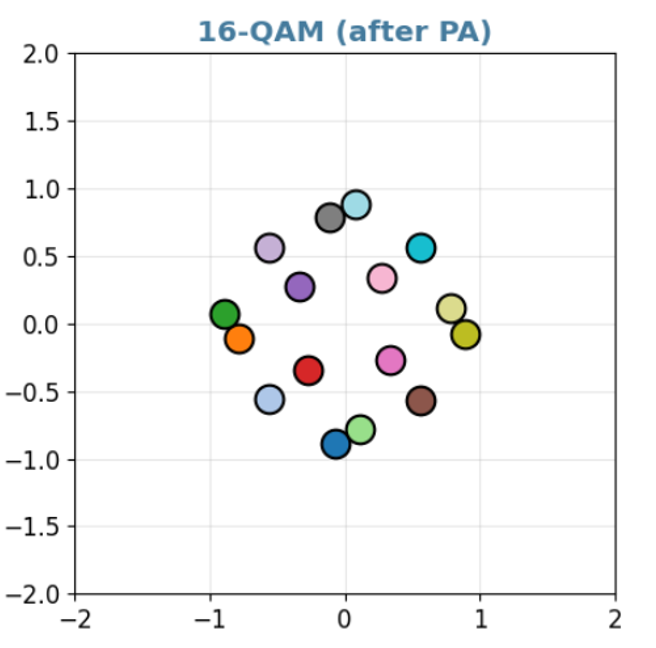
\includegraphics[width=\textwidth]{qam16_after_pa.png}
\caption{PA-distorted 16-QAM constellation.}
\end{subfigure}
\caption{Effect of PA nonlinearity on 16-QAM signal geometry.}
\label{fig:qam16_pa_distortion}
\end{figure}

\section{AutoEncoder Communication Model}
\begin{figure}[H]
\centering
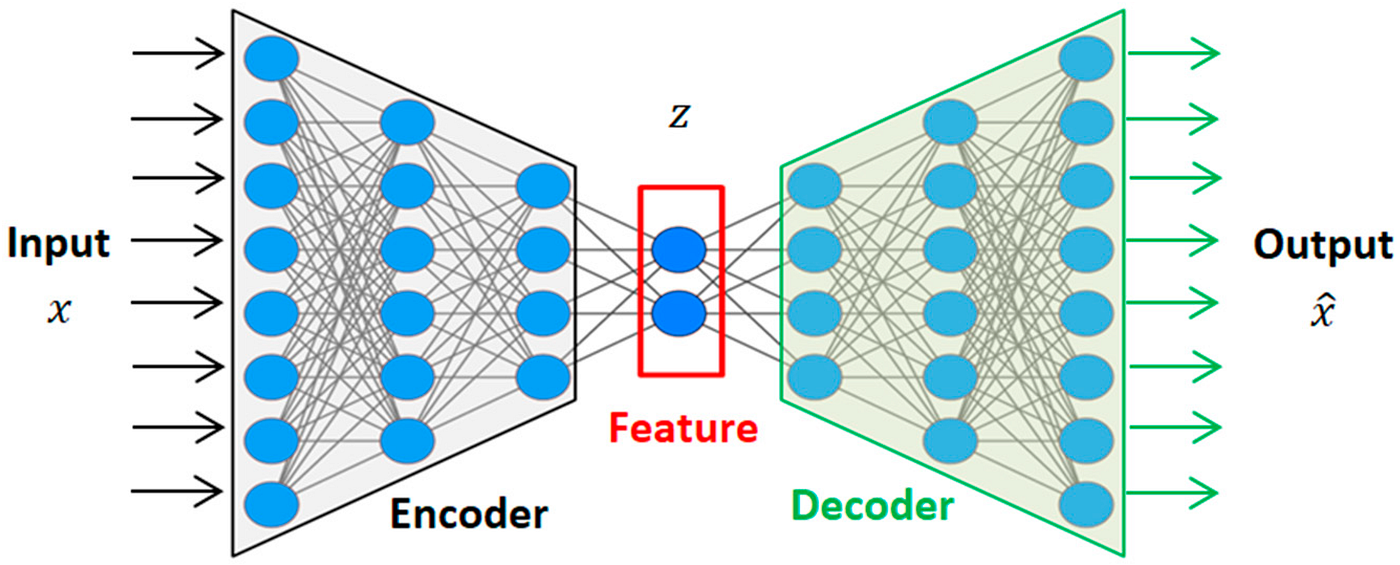
\includegraphics[width=0.88\textwidth]{autoencoder.png}
\caption{AutoEncoder-based learned Modulation and Demodulation model.}
\end{figure}
The autoencoder model has an encoder, a channel layer, and a decoder. The encoder is analogous to a transmitter modulator. The channel layer may be differentiable or simulated. The decoder is analogous to a receiver detector. Training usually minimizes cross-entropy between the transmitted message and the detected message while enforcing an average-power constraint.

Power normalization is essential. Without it, the network could reduce errors simply by increasing transmit energy. A meaningful learned modulation scheme should satisfy the same or comparable power constraint as the baseline. SNR also needs to be varied during training or evaluation, because a constellation optimized for one SNR may not remain optimal across the full operating range.

The autoencoder approach is useful for research because it can reveal how a signal representation changes when the channel changes. For example, under PA nonlinearity, the learned constellation may avoid high-amplitude regions. Under CFO, a multi-symbol model may use temporal structure. Under fading, the receiver may learn robust decision boundaries.

\begin{equation}
m\rightarrow x=f_{\theta}(m),\qquad y=\mathcal{H}(x),\qquad \hat{p}(m|y)=g_{\phi}(y).
\end{equation}
Equation (2.5) describes the autoencoder communication model. The transmitter network $f_\theta$ maps message $m$ to channel input $x$, the channel produces $y$, and the receiver network $g_\phi$ estimates the posterior probability of the message. The parameters $\theta$ and $\phi$ are optimized from data.

\begin{equation}
\mathbb{E}\{|x|^2\}\le P_0.
\end{equation}
Equation (2.6) is the average-power constraint. It prevents the learned transmitter from improving detection simply by increasing transmit energy. Any learned modulation should be compared with a conventional baseline under a comparable power constraint.

\begin{equation}
x_{\mathrm{norm}}=\sqrt{P_0}\frac{x_{\mathrm{raw}}}{\sqrt{\mathbb{E}\{|x_{\mathrm{raw}}|^2\}+\epsilon}}.
\end{equation}
Equation (2.7) is a typical normalization step used to enforce average-power control in neural modulation. If $P_0=1$, it reduces to unit-average-power normalization.

\begin{equation}
\mathcal{L}_{\mathrm{CE}}=-\sum_{m=1}^{M}\mathbf{1}\{m\}\log\hat{p}(m|y).
\end{equation}
Equation (2.8) is the cross-entropy loss commonly used for message classification in communication AutoEncoders. Although useful for training, this loss does not automatically guarantee calibrated bit-level LLRs for iterative decoding.

\begin{equation}
\mathrm{SER}=\frac{N_{\mathrm{sym,err}}}{N_{\mathrm{sym}}}.
\end{equation}
Equation (2.9) defines symbol error rate, which is often used when studying modulation before full channel-code integration.

\section{Non-Ideal Channel Conditions}
\begin{figure}[H]
\centering
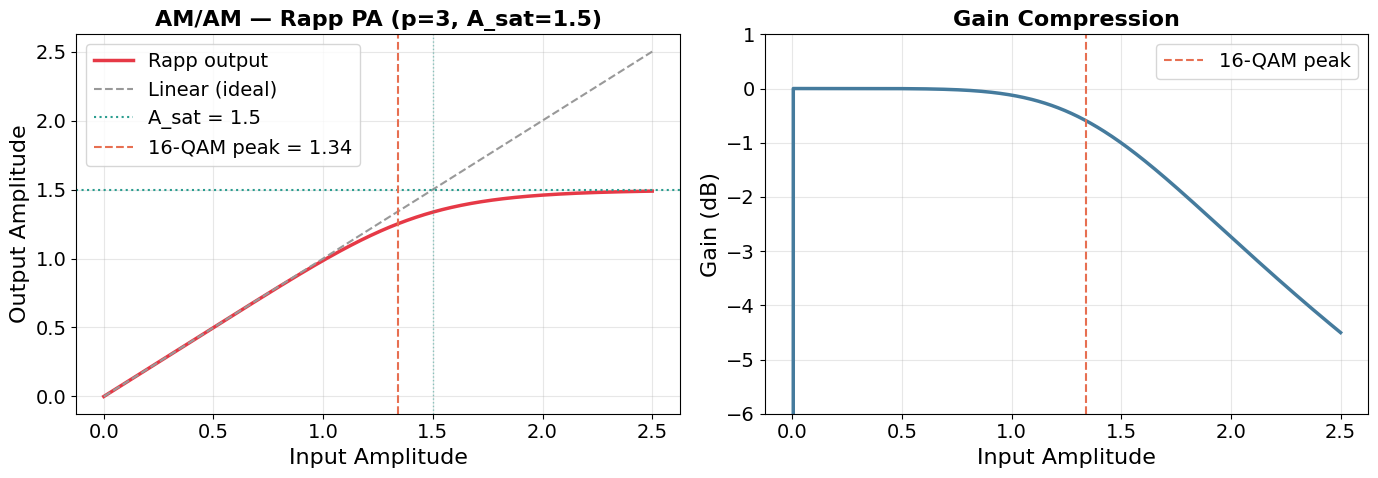
\includegraphics[width=0.78\textwidth]{pa_characteristic.png}
\caption{Rapp-type power-amplifier nonlinearity used in the channel model.}
\end{figure}
\begin{figure}[H]
\centering
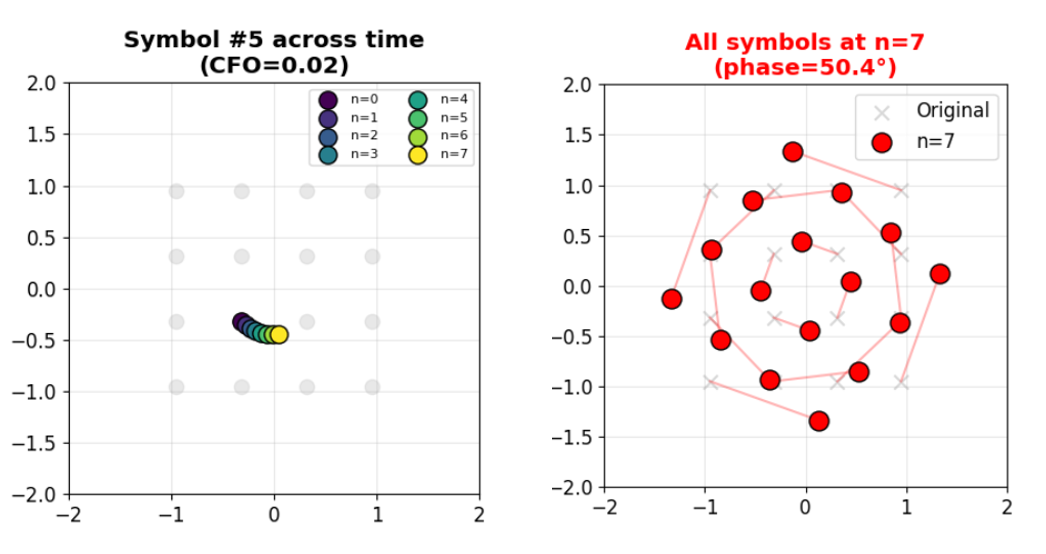
\includegraphics[width=0.78\textwidth]{cfo_effect.png}
\caption{Constellation rotation caused by carrier-frequency offset.}
\end{figure}
Power amplifier nonlinearity is a major practical impairment. A PA is efficient when operated near saturation, but this causes nonlinear amplitude compression. Outer constellation points are compressed more strongly, reducing distances between received clusters. If AM/PM distortion exists, phase is also changed. Learned modulation may improve robustness by shaping symbols away from regions with pronounced compression.

Carrier-frequency offset occurs when transmitter and receiver oscillators are not perfectly aligned. CFO causes phase rotation that accumulates over time. In single-symbol detection, this rotation looks like an unknown phase error. In multi-symbol processing, the receiver can observe the rotation pattern and estimate it implicitly. This motivates sequence-based autoencoder modulation.

Rayleigh fading and ISI represent propagation impairments. Rayleigh fading changes amplitude and phase randomly, while ISI makes the current received sample depend on previous transmitted symbols. A neural receiver can process context and may learn equalization-like behavior. However, this also increases complexity and latency.

\begin{table}[H]
\centering
\caption{Non-ideal channel effects considered for learned Modulation.}
\label{tab:learned_modulation_impairments}
\begin{tabularx}{\textwidth}{p{0.23\textwidth}p{0.30\textwidth}Y}
\toprule
Impairment & Main effect on signal geometry & Relevance to learned Modulation\\
\midrule
PA nonlinearity & Compresses high-amplitude symbols and may introduce amplitude-dependent phase shifts & Encourages the learned constellation to avoid regions strongly distorted by the amplifier\\
CFO & Produces phase rotation that accumulates with time & Motivates multi-symbol neural receivers that exploit temporal phase evolution\\
Rayleigh fading & Randomly changes amplitude and phase of the received signal & Requires robust signal geometry and Demodulation metrics across channel realizations\\
ISI & Couples adjacent transmitted symbols through channel memory & Makes sequence-aware detection more useful than purely memoryless decisions\\
\bottomrule
\end{tabularx}
\end{table}

\begin{equation}
g(r)=\frac{r}{\left[1+\left(r/A_{\mathrm{sat}}\right)^{2p}\right]^{1/(2p)}}.
\end{equation}
Equation (2.10) is a common Rapp-type AM/AM PA model. A\_sat controls saturation amplitude and p controls smoothness. This model explains why high-amplitude constellation points are compressed more strongly.

\begin{equation}
\Phi(r)=\frac{\alpha_{\mathrm{PM}}r^2}{1+\beta_{\mathrm{PM}}r^2}.
\end{equation}
Equation (2.11) is a simple AM/PM distortion model. It indicates that the phase shift can depend on signal amplitude.

\begin{equation}
y_{\mathrm{CFO}}[k]=x[k]e^{j2\pi \Delta f T_s k}+w[k].
\end{equation}
Equation (2.12) represents carrier-frequency offset. The phase rotation grows with symbol index k, which motivates multi-symbol processing because a sequence carries information about the rotation trend.

\begin{equation}
y[n]=\sum_{\ell=0}^{L-1}h[\ell]x[n-\ell]+w[n].
\end{equation}
Equation (2.13) represents a multipath channel with ISI. The received sample depends on multiple transmitted symbols, so memoryless detection may be insufficient. A sequence-based neural receiver can learn to exploit this temporal dependence.

\begin{equation}
h[\ell]\sim\mathcal{CN}(0,\sigma_{\ell}^{2}),\qquad \sum_{\ell}\sigma_{\ell}^{2}=1.
\end{equation}
Equation (2.14) gives a common statistical model for Rayleigh multipath coefficients with normalized average power.

\begin{equation}
\mathcal{L}_{\mathrm{BCE}}=-\frac{1}{K}\sum_{k=1}^{K}\left[b_k\log \hat{b}_k+(1-b_k)\log(1-\hat{b}_k)\right].
\end{equation}
Equation (2.15) is a bit-wise binary cross-entropy objective. It is more directly related to soft bit output than message-level cross-entropy and is therefore relevant for learned Demodulation that supplies LLR-like information to an LDPC decoder.

\section{Simulation Scenarios for Learned Modulation}
\begin{table}[H]
\centering
\caption{Evaluation scenarios for AutoEncoder-based Modulation.}
\label{tab:ae_modulation_scenarios}
\begin{tabularx}{\textwidth}{p{0.25\textwidth}p{0.30\textwidth}Y}
\toprule
Scenario & Compared condition & Main interpretation\\
\midrule
Single-symbol AE & 16-QAM and learned constellation under PA/Rayleigh channel & Evaluates whether learned signal geometry can reduce BER under nonlinear amplitude distortion and fading\\
Multi-symbol AE & Learned sequence model under CFO values of 0.005 and 0.01 & Tests whether temporal context can implicitly compensate accumulated carrier phase rotation\\
AE with neural redundancy & Learned Modulation combined with neural FEC-like redundancy & Provides supporting evidence on the coupling between Modulation, redundancy, and receiver-side inference\\
\bottomrule
\end{tabularx}
\end{table}

\begin{figure}[H]
\centering
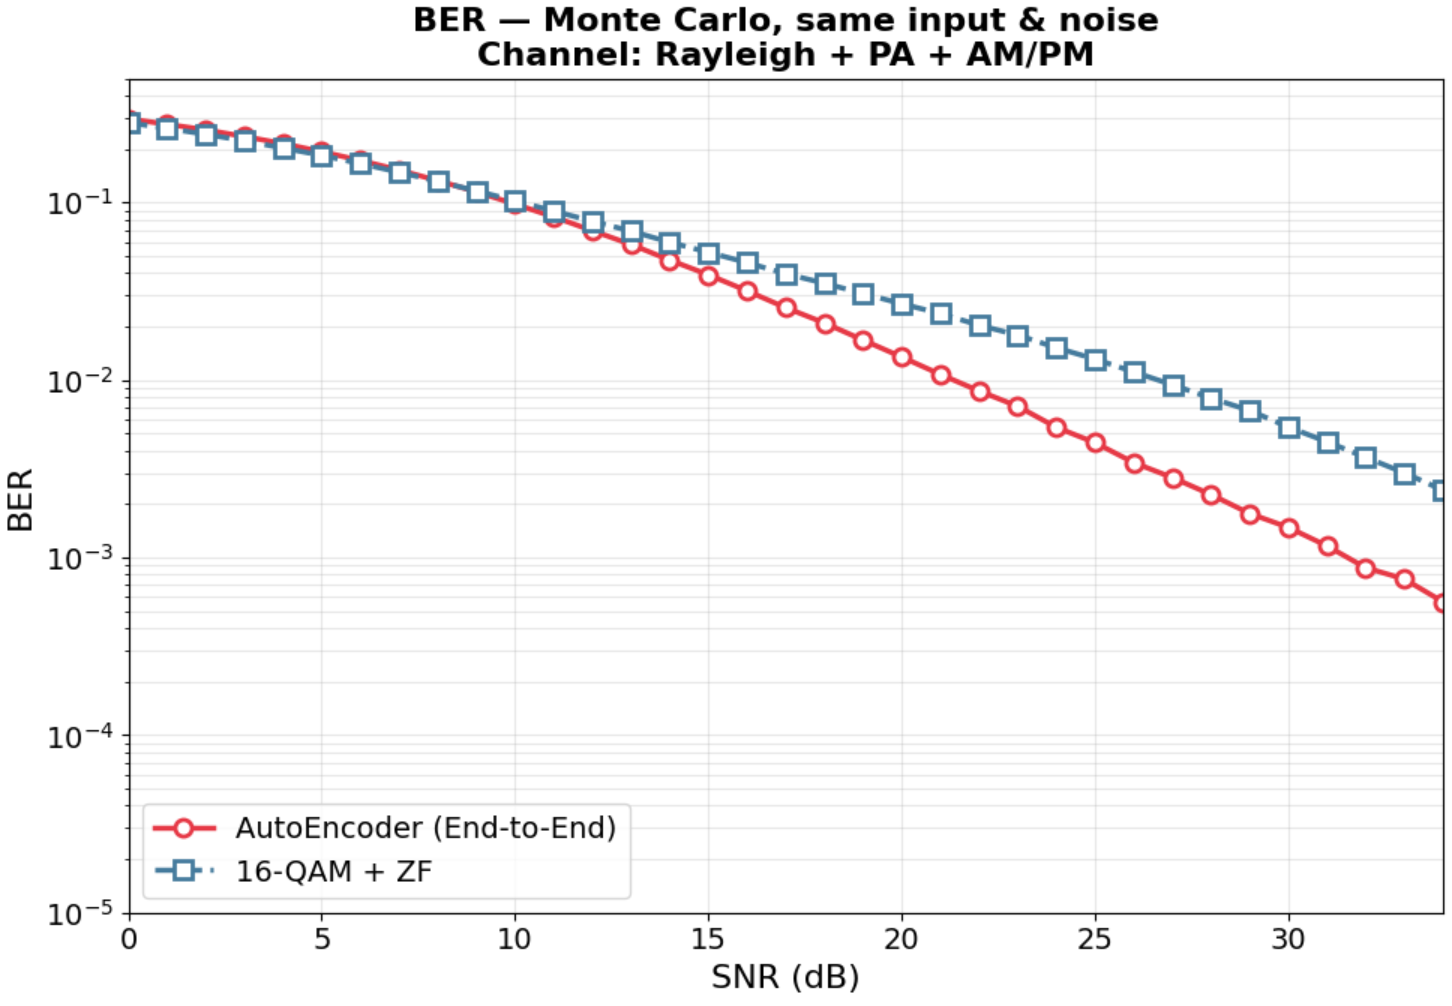
\includegraphics[width=0.86\textwidth]{ae_scenario1_ber.png}
\caption{BER of learned Modulation under PA nonlinearity and Rayleigh fading.}
\end{figure}
\begin{figure}[H]
\centering
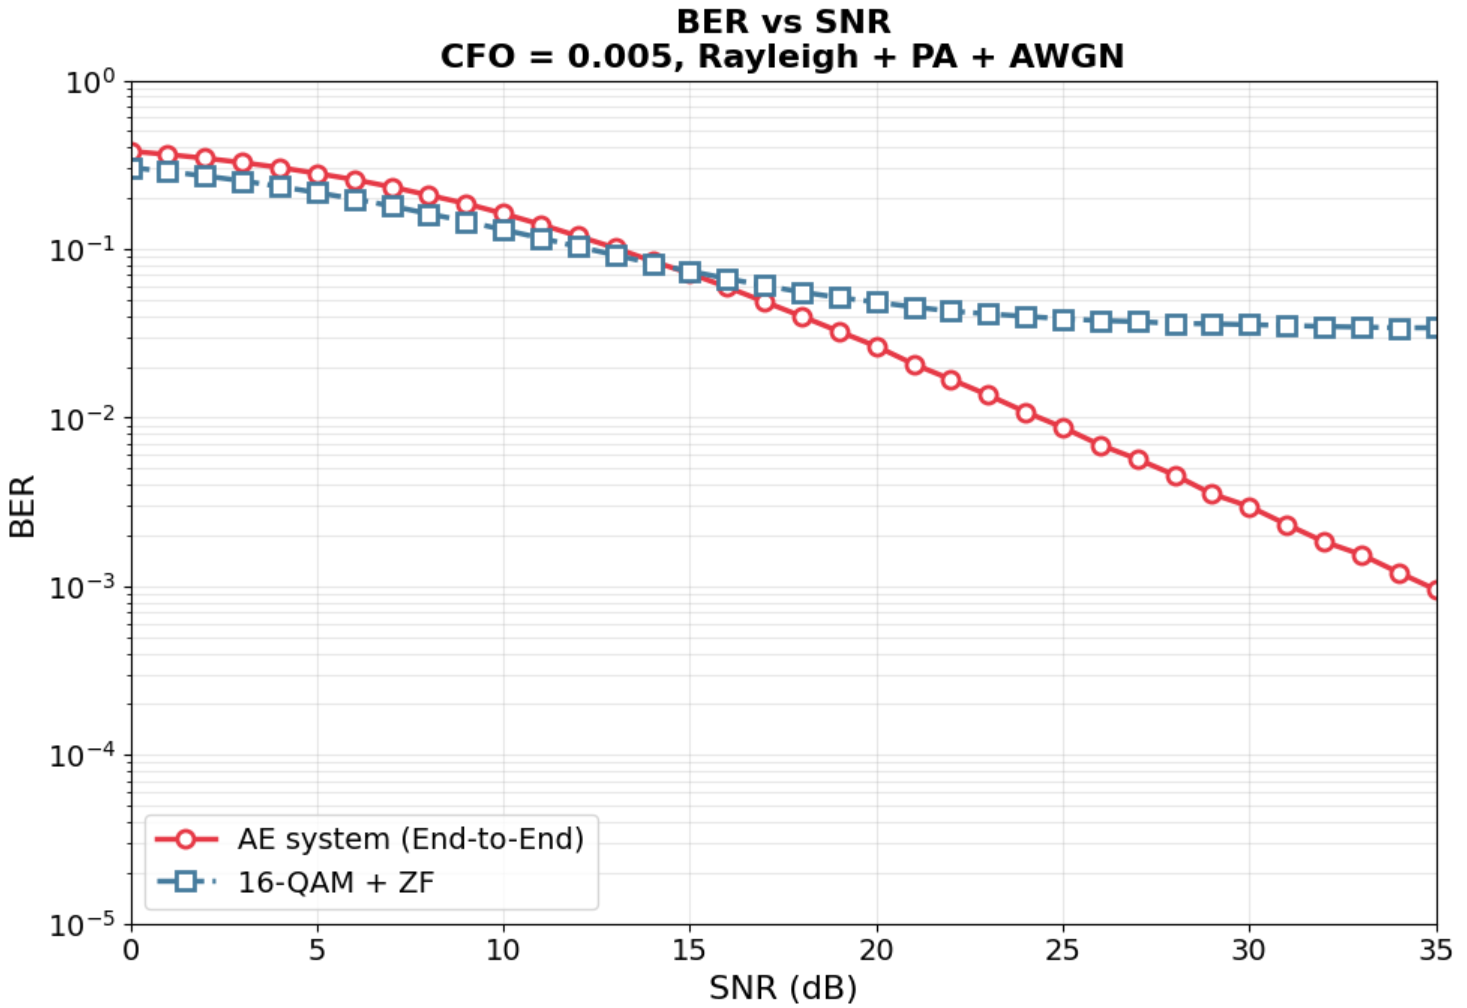
\includegraphics[width=0.86\textwidth]{ae_scenario2_cfo0005.png}
\caption{BER of multi-symbol AutoEncoder Modulation with CFO = 0.005.}
\end{figure}
\begin{figure}[H]
\centering
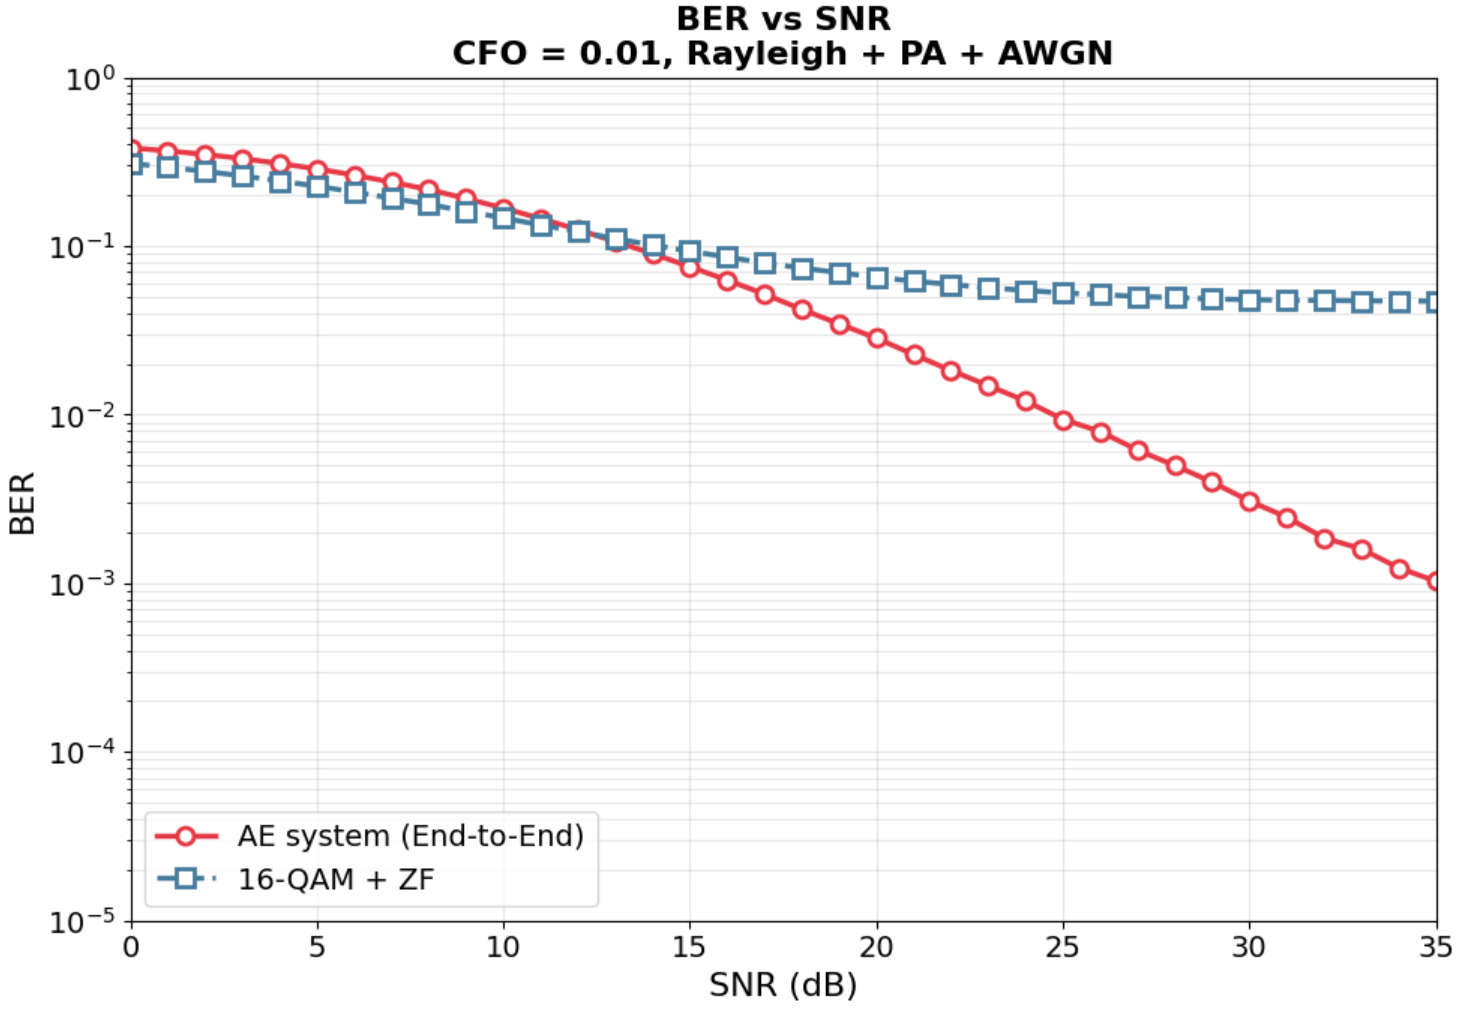
\includegraphics[width=0.86\textwidth]{ae_scenario2_cfo001.png}
\caption{BER of multi-symbol AutoEncoder Modulation with CFO = 0.01.}
\end{figure}
\begin{figure}[H]
\centering
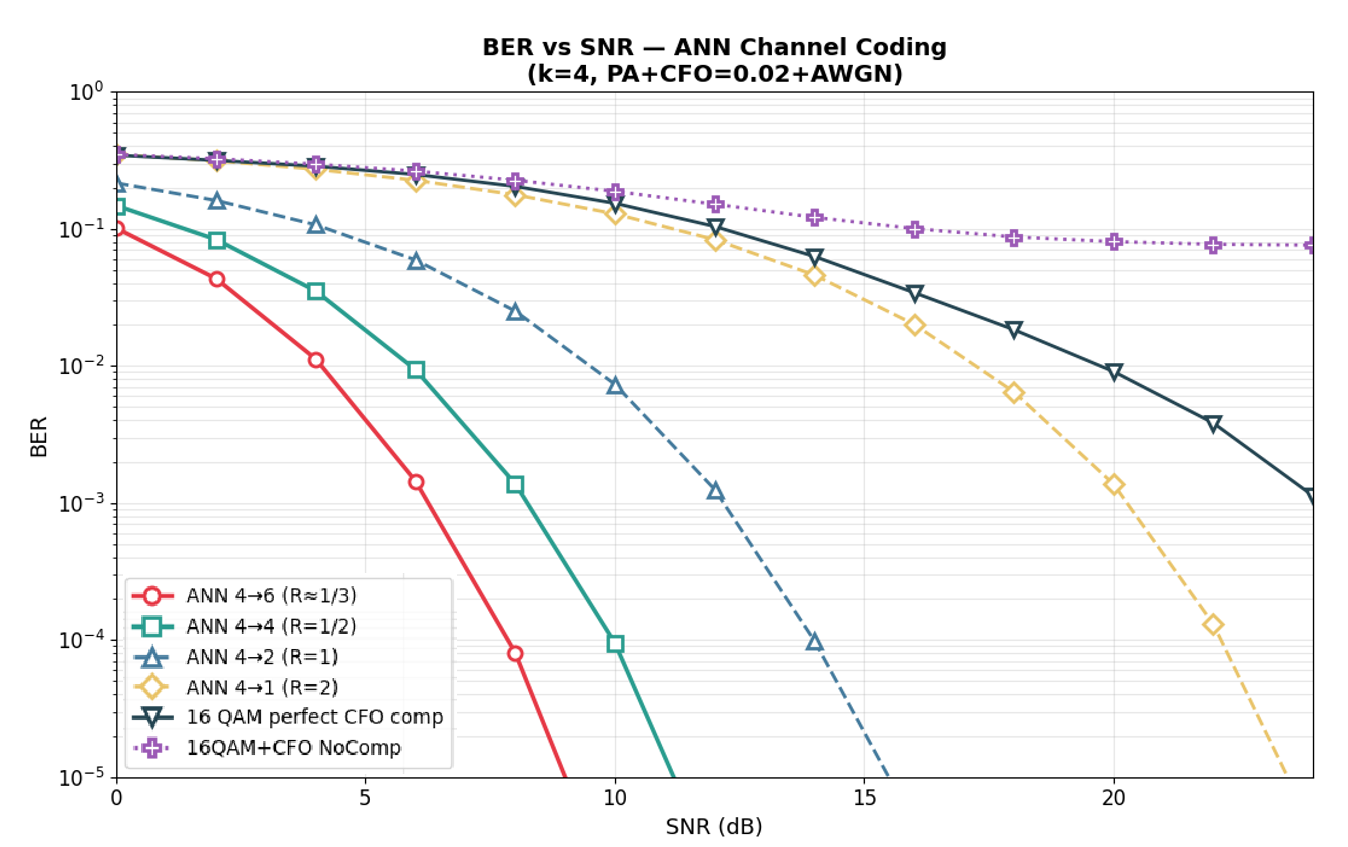
\includegraphics[width=0.86\textwidth]{ae_scenario3_fec.png}
\caption{BER of AutoEncoder Modulation with neural redundancy.}
\end{figure}
The simulation scenarios considered in this chapter include several AutoEncoder configurations. Scenario 1 compares a single-symbol AutoEncoder with 16-QAM under a Rayleigh plus PA channel. This scenario evaluates whether learned constellation shaping can improve BER when nonlinear amplitude distortion is present.

Scenario 2 studies a multiple-symbol AutoEncoder under CFO. Two CFO values are shown in the result figures. This scenario is important because CFO compensation is difficult for a purely memoryless Demodulator. A sequence model can exploit phase evolution across symbols and may reduce the need for an explicit synchronization block.

Scenario 3 studies an AutoEncoder with a neural channel-coding feature. This scenario is best interpreted as a supporting experiment on the relationship between learned Modulation and redundancy, rather than as the central LDPC-decoding result of the thesis.

\section{System Interpretation and Soft-Output Demodulation}
\section{AutoEncoder Modulation as a Supporting Study}
AutoEncoder-based Modulation is included in the thesis because the LDPC decoder operates on the reliability information produced by the receiver front end. If the Modulation and Demodulation process produces biased LLRs, the LDPC decoder may not reach its expected performance even when the decoder algorithm is well designed. Therefore, a study of learned Modulation is relevant as a supporting analysis of the soft-information source in a BIBCM-ID-oriented receiver. The key point is that AutoEncoder Modulation is not presented as the main LDPC-decoding contribution. It is used to examine how a trainable signal mapping and a trainable receiver can adapt to channel impairments that weaken conventional Demodulation.

In a communication AutoEncoder, the transmitter network maps a message or bit pattern to a channel input:
\begin{equation}
  \mathbf{x}=f_\theta(\mathbf{m}),
\end{equation}
the channel produces
\begin{equation}
  \mathbf{y}=\mathcal{H}(\mathbf{x})+\mathbf{w},
\end{equation}
and the receiver network estimates either the transmitted message or the transmitted bits:
\begin{equation}
  \hat{\mathbf{p}}=g_\phi(\mathbf{y}).
\end{equation}
The parameters $\theta$ and $\phi$ are learned by minimizing a loss such as cross-entropy. This formulation resembles an end-to-end communication system, but the interpretation must be precise. If the receiver outputs only a message class, the model is a learned detector. If the receiver outputs bit probabilities or LLR-like values, it becomes more directly relevant to an iterative coded-modulation receiver.

Power normalization is central to a fair comparison. Without a constraint, the transmitter network could reduce the error rate by increasing the signal energy. A typical normalization is
\begin{equation}
  \mathbf{x}_{\mathrm{norm}}
  =
  \sqrt{P_0}
  \frac{\mathbf{x}_{\mathrm{raw}}}
  {\sqrt{\mathbb{E}\{\|\mathbf{x}_{\mathrm{raw}}\|^2\}}},
\end{equation}
which enforces an average-power constraint. When comparing AutoEncoder Modulation with 16-QAM or another baseline, the same effective energy normalization must be used. Otherwise, a BER improvement may reflect higher transmitted power rather than a better signal representation.

The channel layer determines what the AutoEncoder learns. Under AWGN only, a learned constellation may resemble a conventional constellation because Euclidean distance is the dominant design criterion. Under PA nonlinearity, the learned constellation may avoid high-amplitude regions that suffer compression. Under CFO, a sequence-based transmitter and receiver may learn a representation that is robust to phase rotation over time. Under fading and ISI, the receiver may learn equalization-like behavior. These observations explain why the AutoEncoder results are useful for discussing Modulation and Demodulation, even though they are not the central evidence for ANN-assisted LDPC decoding.

\section{PA Nonlinearity and Learned Signal Geometry}
Power-amplifier nonlinearity is one of the most important reasons for studying learned Modulation. Practical transmitters often operate power amplifiers near saturation to improve energy efficiency. Near saturation, the amplifier no longer behaves as a linear gain. A common memoryless model expresses the output as
\begin{equation}
  z=A(r)e^{j(\angle x+\Phi(r))}, \qquad r=|x|,
\end{equation}
where $A(r)$ is the AM/AM conversion and $\Phi(r)$ is the AM/PM conversion. For a Rapp-type AM/AM model,
\begin{equation}
  A(r)=\frac{r}{\left(1+\left(\frac{r}{A_{\mathrm{sat}}}\right)^{2p}\right)^{1/(2p)}}.
\end{equation}
When $r$ is small, $A(r)\approx r$. When $r$ approaches the saturation region, $A(r)$ grows slowly and high-amplitude points are compressed. For square QAM, outer constellation points are affected more strongly than inner points. The received clusters are no longer located at the points assumed by a linear-channel Demodulator.

The effect on LLRs can be severe. A conventional Demodulator may compute
\begin{equation}
  p(y|x)\propto \exp\left(-\frac{|y-hx|^2}{N_0}\right),
\end{equation}
while the actual received sample is closer to
\begin{equation}
  y=hA(|x|)e^{j(\angle x+\Phi(|x|))}+w.
\end{equation}
The mismatch changes both distances and decision boundaries. A learned Modulation scheme can respond by reshaping the constellation before the amplifier so that the post-amplifier points are more separable. Alternatively, a neural receiver can learn the nonlinear inverse or a corrected decision rule.

This interpretation should be kept moderate. Learned Modulation does not automatically solve PA distortion. It depends on the accuracy of the PA model used in training and on whether the operating amplifier matches that model. If the network is trained for one saturation level and tested at another, performance may degrade. Therefore, robust training should randomize the PA model parameters:
\begin{equation}
  A_{\mathrm{sat}}\sim\mathcal{U}(A_{\min},A_{\max}), \qquad
  p\sim\mathcal{U}(p_{\min},p_{\max}).
\end{equation}
This training strategy would encourage the transmitter and receiver to learn a representation that is not overly specialized to one amplifier condition. In the present work, it is treated as a design implication for future development rather than as a claim that the current simulations already cover all hardware variation.

\section{Carrier-Frequency Offset and Sequence-Based Demodulation}
Carrier-frequency offset appears when transmitter and receiver oscillators are not perfectly aligned. In discrete time, the received sample can be modeled as
\begin{equation}
  y[k]=x[k]e^{j(2\pi\epsilon k+\varphi_0)}+w[k],
\end{equation}
where $\epsilon$ is the normalized CFO and $\varphi_0$ is the initial phase. A memoryless Demodulator observes only one rotated symbol at a time. If the phase is unknown, the point may appear closer to the wrong decision region. A sequence-based receiver observes multiple samples:
\begin{equation}
  \mathbf{y}_{k:k+T-1}=[y[k],y[k+1],\ldots,y[k+T-1]],
\end{equation}
and can exploit the fact that the phase rotation evolves systematically with $k$.

This explains why the multi-symbol AutoEncoder scenario is relevant. A learned receiver with sequence input can implicitly estimate or compensate a rotation trend. The benefit is not merely that a neural network is used; the benefit comes from providing temporal context to the receiver. In classical communication systems, CFO is normally handled by synchronization algorithms. The AutoEncoder result can be interpreted as evidence that a neural receiver can absorb part of the synchronization burden under a controlled scenario.

The complexity trade-off must also be stated. Sequence processing increases latency and memory because the receiver uses a window of samples rather than a single symbol. If the sequence length is $T$ and the hidden dimension is $d_h$, the computational cost can grow approximately with $T d_h$ for simple feed-forward processing and more for recurrent or attention-based models. Therefore, a sequence-based neural receiver is useful only when the performance gain justifies the increased latency and complexity.

For BIBCM-ID relevance, CFO affects the LLRs delivered to the LDPC decoder. If CFO is not corrected, the Demodulation block may produce low-confidence or wrong-confidence messages. A learned Demodulator that is robust to CFO could provide better soft information. However, to support iterative decoding, it should output bit-level reliability values rather than only message decisions. A possible interface is
\begin{equation}
  \hat{L}_k=g_\phi(\mathbf{y}_{k:k+T-1},L_{A,k}),
\end{equation}
where $L_{A,k}$ represents a priori information from the decoder. This equation is a design direction for learned soft Demodulation; it shows how AutoEncoder ideas can be made compatible with BIBCM-ID principles.

\section{LLR Calibration for Neural Demodulation}
The most important scientific bridge between AutoEncoder Modulation and LDPC decoding is LLR calibration. A neural receiver trained with cross-entropy may output probabilities that are useful for classification but not perfectly calibrated \cite{guo2017}. Calibration means that when a receiver outputs probability $0.9$, the event should be correct approximately 90 percent of the time over many samples with similar confidence. Poor calibration is harmful for iterative decoding because the LDPC decoder uses probability magnitudes as reliability weights.

For bit $b_k$, a neural receiver may output $\hat{p}_k=P(b_k=1|\mathbf{y})$. The corresponding LLR is
\begin{equation}
  \hat{L}_k=\log\frac{\hat{p}_k}{1-\hat{p}_k}.
\end{equation}
If $\hat{p}_k$ is overconfident, $|\hat{L}_k|$ becomes too large. If the sign is wrong, a large magnitude can mislead the LDPC decoder. A simple calibration method is temperature scaling:
\begin{equation}
  \hat{p}_k(T)=\sigma\left(\frac{z_k}{T}\right),
\end{equation}
where $z_k$ is the neural logit, $\sigma(\cdot)$ is the sigmoid function, and $T>0$ is a calibration temperature. If $T>1$, the output probabilities become less confident. If $T<1$, they become sharper. The temperature can be selected on a validation set by minimizing negative log-likelihood.

Calibration can also be evaluated with the Brier score:
\begin{equation}
  \mathrm{Brier}=\frac{1}{N}\sum_{n=1}^{N}(\hat{p}_n-b_n)^2,
\end{equation}
or with reliability diagrams that compare predicted confidence with empirical accuracy. These metrics are not substitutes for BER, but they explain whether the receiver is producing usable soft information. For an iterative coded-modulation system, a receiver with slightly worse hard-decision accuracy but better calibrated LLRs may sometimes support better decoding than an overconfident classifier.

This point is particularly important for the thesis title. The central object is LDPC decoding, and LDPC decoding depends on soft information. AutoEncoder Modulation is therefore defensible as a supporting topic only when it is linked to soft-output Demodulation and trainable receiver interfaces \cite{cammerer2020}. The thesis makes that link explicit: learned Modulation is not discussed as an isolated deep-learning demonstration, but as a way to study how channel-aware signal representation and neural receiver processing may improve the reliability information supplied to the decoder.

\section{Quality Criteria for Interpreting AutoEncoder Results}
AutoEncoder communication results should be interpreted using several criteria. The first criterion is the baseline. A learned constellation should be compared with a conventional scheme under the same power constraint, channel model, SNR definition, and receiver information. If the baseline receiver lacks channel-state information while the neural receiver implicitly learns it from training, the comparison may be unfair. Therefore, the presented figures are treated as evidence of feasibility and trend, not as a general performance claim.

The second criterion is the training distribution. If the model is trained and tested on exactly the same impairment parameters, the result measures interpolation within a narrow condition. A stronger result would test random PA parameters, multiple CFO values, fading distributions not seen during training, and different SNR ranges. This does not invalidate the presented results; it defines their scope.

The third criterion is the output interface. A message-classification AutoEncoder is useful for studying learned signal geometry. A BIBCM-ID-compatible neural Demodulator must go further and produce bit-level soft information:
\begin{equation}
  \mathbf{\hat{L}}=[\hat{L}_1,\ldots,\hat{L}_m].
\end{equation}
If iterative feedback is used, the neural Demodulator should also accept a priori information from the decoder. Without this interface, the receiver remains a learned detector rather than an iterative Demodulation component.

The fourth criterion is complexity. A neural receiver with a large number of layers may improve a BER curve but may not be attractive for a practical receiver. Complexity should be evaluated through parameter count, multiply-accumulate operations, latency, memory access, and quantization robustness. These criteria mirror the ANN-assisted LDPC discussion: a neural method is most valuable when it improves or preserves performance while maintaining a realistic implementation path.

The fifth criterion is interpretability. Classical Modulation designs can be explained through Euclidean distance, Gray labeling, PAPR, and likelihood functions. Learned Modulation should be analyzed using similar concepts where possible. For example, if the learned constellation moves points away from the PA saturation region, this can be explained through AM/AM distortion. If a sequence receiver improves under CFO, this can be explained through temporal phase structure. Such interpretation makes the AutoEncoder part more suitable for an engineering thesis.

\section{Connection Between the Two Research Directions}
The two research directions in the thesis are connected by soft-information quality. The ANN-assisted LDPC decoder acts inside the channel decoder. It modifies the way reliability messages are combined under parity constraints. The AutoEncoder Modulation study acts before the decoder. It explores how the transmitted representation and receiver observation processing affect the reliability values that enter the decoder. Both directions therefore address the same system-level concern from complementary positions.

This connection can be written compactly. Let $\mathbf{L}_{\mathrm{dem}}$ denote the LLR vector produced by the Demodulation block and let $\mathcal{D}_\theta$ denote an ANN-assisted LDPC decoder. The decoded estimate is
\begin{equation}
  \hat{\mathbf{u}}=\mathcal{D}_\theta(\mathbf{L}_{\mathrm{dem}}).
\end{equation}
The decoder performance depends on both $\mathcal{D}_\theta$ and the distribution of $\mathbf{L}_{\mathrm{dem}}$. AutoEncoder Modulation changes this distribution by changing the signal mapping or receiver processing:
\begin{equation}
  \mathbf{L}_{\mathrm{dem}}=g_\phi(\mathbf{y},\mathbf{L}_A).
\end{equation}
Thus, the AutoEncoder study is relevant because it examines the upstream conditions under which the ANN-assisted LDPC decoder operates.

This connection should be interpreted without overstatement. The present analysis does not require a claim that both neural components have been jointly optimized. It is sufficient and more scientifically defensible to show that the LDPC decoder contribution is direct, while the AutoEncoder Modulation analysis identifies a compatible supporting direction. This framing resolves the apparent mismatch between the thesis title and Chapter 3. Chapter 3 is not a detour from LDPC decoding; it studies how Modulation and Demodulation affect the soft information that LDPC decoding consumes.

\section{Soft-Output Neural Demodulation Requirements}
A learned Demodulation block becomes relevant to LDPC decoding only when its output can be used as decoder input. A classifier that outputs a message index is not sufficient for iterative coded modulation. The LDPC decoder requires bit-level reliability. Therefore, a neural Demodulator should output either calibrated bit probabilities or directly output LLR values:
\begin{equation}
  \mathbf{\hat{L}}=
  [\hat{L}_1,\hat{L}_2,\ldots,\hat{L}_m]^T.
\end{equation}
If the neural receiver outputs logits $\mathbf{z}$, one possible conversion is
\begin{equation}
  \hat{L}_k=z_k,
\end{equation}
when the logits are trained as log-odds for bit $k$. If the receiver outputs probabilities, the conversion is
\begin{equation}
  \hat{L}_k=\log\frac{\hat{p}_k}{1-\hat{p}_k}.
\end{equation}
The probability must be clipped away from zero and one in implementation to avoid infinite LLRs:
\begin{equation}
  \hat{p}_{k,\epsilon}=\min(1-\epsilon,\max(\epsilon,\hat{p}_k)).
\end{equation}
This simple numerical detail matters because one overconfident wrong LLR can dominate several iterations of LDPC decoding.

A soft-output neural Demodulator can be trained with bit-wise binary cross-entropy:
\begin{equation}
  \mathcal{L}_{\mathrm{BCE}}=
  -\frac{1}{m}\sum_{k=1}^{m}
  \left[
  b_k\log\hat{p}_k+(1-b_k)\log(1-\hat{p}_k)
  \right].
\end{equation}
This loss is closer to LDPC input requirements than message-level cross-entropy. However, BCE still does not guarantee perfect calibration. Therefore, a validation set should be used to evaluate whether the predicted probabilities correspond to empirical reliability. Calibration can be improved by temperature scaling, isotonic regression, or training objectives that penalize overconfidence.

If iterative feedback is considered, the Demodulator should also accept a priori information from the decoder:
\begin{equation}
  \mathbf{\hat{L}}^{(t)}
  =
  g_\phi(\mathbf{y},\mathbf{L}_A^{(t)}).
\end{equation}
The extrinsic output is then
\begin{equation}
  \mathbf{L}_E^{(t)}=\mathbf{\hat{L}}^{(t)}-\mathbf{L}_A^{(t)}.
\end{equation}
This equation is the neural analogue of classical iterative Demodulation. It shows how AutoEncoder ideas can be connected to BIBCM-ID without overstating the current results. The present thesis uses AutoEncoder Modulation as a supporting study, but the mathematical interface for future soft-output Demodulation is already clear.

\section{Learned Demapper Architectures and Engineering Trade-Offs}
Several neural architectures can be used for learned Demodulation. A memoryless multilayer perceptron can process the real and imaginary parts of one received symbol:
\begin{equation}
  \mathbf{r}_t=[\Re(y_t),\Im(y_t),\Re(h_t),\Im(h_t),\sigma^2]^T.
\end{equation}
This architecture is simple and low-latency, but it cannot exploit temporal structure such as CFO evolution or ISI memory. A sequence model can process a window of samples:
\begin{equation}
  \mathbf{R}_t=[\mathbf{r}_{t-L},\ldots,\mathbf{r}_t,\ldots,\mathbf{r}_{t+L}],
\end{equation}
which improves the ability to compensate memory and phase drift at the cost of latency.

Convolutional neural networks can exploit local temporal patterns with shared filters. Recurrent neural networks can model sequential dependence but may be harder to parallelize. Attention-based models can learn long-range dependence, but they may be too expensive for a low-latency receiver unless the sequence length is small. For a master's thesis focused on LDPC decoding, it is not necessary to implement all architectures. It is more useful to explain which architectural properties matter: soft-output capability, calibration, latency, parameter count, and compatibility with a priori information.

The engineering trade-off can be summarized as
\begin{equation}
  \mathcal{J}
  =
  \mathrm{BER}
  +\lambda_1 C_{\mathrm{comp}}
  +\lambda_2 T_{\mathrm{lat}}
  +\lambda_3 M_{\mathrm{mem}},
\end{equation}
where $C_{\mathrm{comp}}$ is computational cost, $T_{\mathrm{lat}}$ is latency, and $M_{\mathrm{mem}}$ is memory. The weights $\lambda_1,\lambda_2,\lambda_3$ depend on the target receiver. This expression does not define a universal objective, but it makes clear that BER alone is not enough for engineering evaluation.

The learned Demodulator must also respect signal normalization. If the transmitter network changes the constellation, the receiver should know the effective scaling or learn it robustly. If the channel gain varies, the receiver may need CSI or an implicit channel-estimation mechanism. If the Demodulator is trained with perfect CSI but deployed with imperfect CSI, the resulting LLRs may be overconfident. Therefore, training should include the same uncertainty expected in deployment:
\begin{equation}
  \hat{h}=h+e_h, \qquad e_h\sim\mathcal{CN}(0,\sigma_h^2).
\end{equation}
This channel-estimation error can be added during training so that the learned receiver does not depend unrealistically on perfect channel knowledge.

\section{Why Chapter 3 Strengthens Rather Than Dilutes the Thesis}
The title emphasizes ANN utilization in LDPC decoding for BIBCM-ID systems. A narrow interpretation would include only the channel decoder. However, BIBCM-ID is an iterative receiver architecture, and the LDPC decoder is driven by soft information produced by Demodulation. Therefore, a technically mature treatment explains not only the decoder update but also the nature of the input messages that the decoder receives. Chapter 3 serves this purpose.

The chapter does not change the main contribution. The direct contribution remains the ANN-assisted check-node update in LDPC decoding. The AutoEncoder material supports the system context by analyzing how learned Modulation and Demodulation can affect the reliability of the decoder input. This framing is stronger than presenting AutoEncoder Modulation as an unrelated second topic. It connects both research directions through one technical theme: the generation, transformation, and use of soft information.

If Chapter 3 were written as a general deep-learning communication chapter, it would appear misaligned with the title. The revised structure instead explains that learned Modulation is relevant because it changes the distribution and calibration of LLRs. The LDPC decoder is then understood as the downstream component whose performance depends on those LLRs. The discussion is therefore system-aware while keeping the LDPC decoder as the center of the thesis.

The correct level of conclusion is also important. AutoEncoder Modulation is presented as evidence and analysis for channel-aware signal mapping under non-ideal conditions, not as a finished solution to BIBCM-ID receiver design. The next technical step would be a soft-output neural Demodulator that produces calibrated bit LLRs and can exchange extrinsic information with an LDPC decoder. This is a natural continuation of the current contribution.

\section{Recommended Validation Extension}
For a stronger continuation of the work, the following validation path is technically coherent. First, evaluate the ANN-assisted LDPC decoder using BPSK-AWGN input to isolate the check-node approximation. Second, evaluate the same decoder using LLRs produced by conventional high-order Demodulation under BIBCM-ID-like interleaving. Third, evaluate a learned Demodulator that outputs calibrated bit LLRs under PA and CFO impairments. Fourth, compare the LDPC decoder with and without the ANN check-node update under the same Demodulation input.

This staged validation has a clear reason. It separates the decoder contribution from the Modulation/Demodulation contribution. If performance changes after replacing the check-node update, the effect can be attributed to the decoder. If performance changes after replacing the Demodulator, the effect can be attributed to the soft-information source. If both are changed simultaneously, interpretation becomes more difficult.

The staged path can be expressed as four receiver configurations:
\begin{equation}
  \mathcal{R}_1=(\mathrm{Conventional\ Demodulation},\mathrm{SPA\ LDPC}),
\end{equation}
\begin{equation}
  \mathcal{R}_2=(\mathrm{Conventional\ Demodulation},\mathrm{ANN\ LDPC}),
\end{equation}
\begin{equation}
  \mathcal{R}_3=(\mathrm{Learned\ Demodulation},\mathrm{SPA\ LDPC}),
\end{equation}
\begin{equation}
  \mathcal{R}_4=(\mathrm{Learned\ Demodulation},\mathrm{ANN\ LDPC}).
\end{equation}
The current thesis provides the strongest evidence for $\mathcal{R}_2$ and supporting analysis for the learned-Demodulation side. This statement is precise, defensible, and aligned with the available materials.

\section{Consistency Check of the Three-Chapter Structure}
From an examination viewpoint, the three chapters should form one argument rather than three separate reports. Chapter 1 defines the BIBCM-ID context and explains why Modulation, Demodulation, interleaving, and channel decoding are coupled through soft information. Chapter 2 then focuses on the main contribution: ANN-assisted LDPC decoding through local check-node message approximation. Chapter 3 supports the same system context by analyzing how learned Modulation and Demodulation can affect the reliability values supplied to the LDPC decoder. This ordering keeps the thesis title credible because the decoder remains the central contribution, while the AutoEncoder material is used to explain the upstream source of decoder input quality.

The main scientific boundary is the level of claim. AutoEncoder Modulation is not used as evidence that the whole BIBCM-ID receiver has already been improved. The structure uses three levels of claim. The first level is established theory: LDPC decoding, BICM-ID/BIBCM-ID soft-information exchange, and classical Modulation/Demodulation. The second level is the implemented or directly analyzed contribution: ANN-assisted LDPC check-node processing. The third level is supporting investigation: learned Modulation under non-ideal channels and its relevance to soft-output Demodulation. These levels remain distinct throughout the thesis.

Complexity reduction is treated through concrete criteria: removal of nonlinear SPA operations, parameter count, weight sharing, quantization, average iteration count, and latency. This makes the argument more robust. The ANN is presented as a practical approximation of a costly nonlinear update with a measurable trade-off between performance and implementation cost, rather than as a universally simpler decoder.

The evaluation framework also avoids relying only on BER. The expanded discussion includes FER, average iteration count, simulation length, LLR calibration, and validation over SNR ranges. These criteria reduce the possibility of selecting only the metric that favors the proposed method. For a technical master's thesis, this balanced evaluation framework is often as important as the numerical curve itself.

The final consistency requirement is terminology. The text uses Modulation for the transmitter-side mapping, Demodulation for the receiver-side soft metric computation, LDPC decoding for parity-check message passing, and AutoEncoder Modulation for the learned signal-mapping study. Maintaining these terms consistently reduces ambiguity and helps the reader see why Chapter 3 belongs in the thesis without changing the main LDPC-decoding emphasis.


\subsection{Interpretation and BIBCM-ID Relevance}
The AutoEncoder results are interpreted as evidence that learned Modulation and Demodulation can adapt to selected channel impairments. They do not establish that learned constellations should replace standardized modulation in general-purpose systems. Conventional constellations provide interoperability, simple implementation, and predictable Demodulation rules. Learned modulation offers adaptability, but its benefit depends on the channel model, training distribution, power constraint, receiver structure, and calibration of soft outputs.

The reason this topic is included in a thesis centered on ANN-assisted LDPC decoding is the soft-information interface. In BIBCM-ID, the LDPC decoder does not receive ideal bits; it receives reliability values produced by the Demodulation block after interleaving and channel observation. If PA distortion, CFO, fading, or ISI makes conventional LLRs biased, the LDPC decoder receives messages with reduced reliability. A study of learned Modulation/Demodulation is therefore relevant because it analyzes the upstream source of the information consumed by the LDPC decoder.

The main thesis contribution remains the ANN-assisted LDPC check-node update. This contribution is directly located inside the LDPC decoder and can reduce computational burden by approximating the nonlinear SPA check-node operation with a compact neural model. Under the evaluated conditions, the most defensible interpretation is that the ANN approximation can preserve decoding behavior close to SPA while reducing the cost of nonlinear operations; reliability-aware labeling may improve BER in selected simulations, but the broader engineering value is the balance between decoding quality and implementation complexity.

AutoEncoder-based Modulation is presented as a complementary investigation. It supports the overall BIBCM-ID context by showing how learned signal representations may produce observations that are more robust under non-ideal channels. The chapter therefore connects AutoEncoder results to Modulation, Demodulation, and LLR quality, while keeping the primary LDPC-decoding contribution clearly centered on ANN-assisted check-node processing.

A technically consistent interpretation must separate final BER from message quality. A neural receiver can reduce hard-decision errors in a simulated scenario while still producing probabilities that are not well calibrated for iterative decoding. For this reason, future development of learned Demodulation should emphasize bit-level probabilities, LLR calibration, and robustness across SNR and channel variations. These requirements are stated as design implications for later research on learned soft Demodulation.

\section{Chapter Conclusion}
This chapter has analyzed deep learning for intelligent Modulation and Demodulation under non-ideal wireless channels. The discussion began from the observation that conventional constellations and Demodulation rules are usually derived under simplified assumptions such as AWGN, linear amplification, or separately compensated synchronization errors. In practical wireless channels, PA nonlinearity, CFO, fading, and ISI can distort the received constellation and reduce the reliability of the LLR values passed to the channel decoder.

AutoEncoder-based Modulation is therefore examined as a supporting study of the BIBCM-ID soft-information chain. The transmitter network, differentiable or simulated channel layer, and receiver network provide a framework for learning signal representations adapted to specific impairments. The simulation scenarios indicate that learned representations can reduce the effect of PA compression, exploit temporal structure under CFO, and support receiver processing in channels with memory. These results should not be read as a general replacement for standardized Modulation, because their validity depends on the training distribution, baseline fairness, power normalization, and receiver complexity.

The main relevance of this chapter to the thesis title lies in LLR quality. LDPC decoding performance depends on the reliability values produced before the decoder, not only on the internal decoding algorithm. A learned Modulation/Demodulation block becomes compatible with BIBCM-ID only when it can provide calibrated bit-level soft information and, in an iterative setting, accept a priori information from the decoder. The chapter therefore strengthens the system interpretation of the ANN-LDPC contribution: Chapter 2 explains how learned front-end processing may affect the reliability messages entering the decoder, while Chapter 3 improves or approximates the processing of reliability messages inside the decoder.

\chapter[\textbf{ANN-ASSISTED LDPC DECODING}]{ANN-ASSISTED LDPC DECODING}
\section{LDPC Decoding and the Check-Node Update}
LDPC decoding is usually described on a Tanner graph containing variable nodes and check nodes. Variable nodes represent code bits, while check nodes represent parity constraints. In each iteration, messages are exchanged along graph edges. The VN update combines channel reliability with incoming check-node messages. The CN update combines incoming variable-node messages to produce parity-consistency information.

The Sum-Product Algorithm is the classical probabilistic decoding method. In the LLR domain, the CN update requires nonlinear transformations involving tanh or equivalent logarithmic functions. These operations are accurate but costly in hardware. In a high-throughput decoder, millions of CN updates may be computed per second. Reducing the cost of this operation is therefore a practical engineering problem.

Min-Sum reduces this cost by using the sign product and the minimum magnitude of incoming messages. It captures the dominant behavior of the CN update but ignores the nonlinear correction contained in SPA. Normalized and offset variants add empirical correction factors, but the correction is still fixed. The ANN approach can be viewed as a learnable correction~function.

\begin{equation}
\mathbf{H}\mathbf{c}^{T}=\mathbf{0}.
\end{equation}
Equation (3.1) is the parity-check condition for an LDPC code. The sparse parity-check matrix H defines the Tanner graph. A valid codeword c should satisfy all parity constraints. Decoding can therefore be interpreted as the process of finding the most likely codeword that satisfies these constraints.

\begin{equation}
L_{\mathrm{ch},j}=\ln\frac{p(y_j|c_j=1)}{p(y_j|c_j=0)}.
\end{equation}
Equation (3.2) gives the channel LLR used to initialize the LDPC decoder. For the BPSK/AWGN derivation under the LLR convention above, the equivalent binary mapping is $c_j=1\mapsto +1$ and $c_j=0\mapsto -1$. With $y_j=s_j+n_j$ and $n_j\sim\mathcal{N}(0,\sigma^2)$,
\begin{equation*}
L_{\mathrm{ch},j}=\frac{2y_j}{\sigma^2}.
\end{equation*}
If the alternative BPSK mapping $0\mapsto +1$, $1\mapsto -1$ is used, the sign of the channel LLR must be reversed. The exact scaling affects message magnitudes and therefore iterative convergence.

\begin{equation}
L_{j\rightarrow i}^{(t)}=L_{\mathrm{ch},j}+\sum_{i'\in\mathcal{N}(j)\setminus i}L_{i'\rightarrow j}^{(t-1)}.
\end{equation}
Equation (3.3) is the variable-node update in the LLR domain. The message from variable node j to check node i is the channel reliability plus all incoming check-node messages except the one from check node i. This exclusion is necessary to preserve the extrinsic-information principle.

\begin{equation}
L_{i\rightarrow j}^{(t)}=
2\tanh^{-1}\!\prod_{j'\in\mathcal{N}(i)\setminus j}\tanh\!\left(\frac{L_{j'\rightarrow i}^{(t)}}{2}\right).
\end{equation}
Equation (3.4) is the SPA check-node update. It is accurate but computationally expensive because it contains hyperbolic tangent and inverse hyperbolic tangent operations. This is the main mathematical motivation for replacing or approximating the CN update by a compact ANN.

\begin{equation}
L_{i\rightarrow j}^{(t)}\approx
\left(\prod_{j'\ne j}\mathrm{sign}(L_{j'\rightarrow i}^{(t)})\right)
\min_{j'\ne j}|L_{j'\rightarrow i}^{(t)}|.
\end{equation}
Equation (3.5) shows the Min-Sum approximation. It keeps the sign product and minimum magnitude behavior of SPA, but discards nonlinear correction terms. This greatly reduces complexity but can degrade decoding~performance.

\begin{equation}
L_{i\rightarrow j,\mathrm{NMS}}^{(t)}=\alpha L_{i\rightarrow j,\mathrm{MS}}^{(t)},\qquad 0<\alpha\le 1.
\end{equation}
Equation (3.6) gives the normalized Min-Sum correction. The scalar $\alpha$ reduces overestimated message magnitudes and partially compensates for the approximation error of Min-Sum.

\begin{equation}
L_{i\rightarrow j,\mathrm{OMS}}^{(t)}=\mathrm{sign}(L_{\mathrm{MS}})\max(|L_{\mathrm{MS}}|-\beta,0).
\end{equation}
Equation (3.7) gives the offset Min-Sum correction. The offset $\beta$ subtracts a fixed reliability margin from the Min-Sum magnitude.

\begin{equation}
L_{\mathrm{APP},j}^{(t)}=L_{\mathrm{ch},j}+\sum_{i\in\mathcal{N}(j)}L_{i\rightarrow j}^{(t)}.
\end{equation}
Equation (3.8) defines the a posteriori LLR used for the hard decision after one decoding iteration.

\begin{equation}
\hat{c}_j=\begin{cases}1,&L_{\mathrm{APP},j}\ge 0,\\0,&L_{\mathrm{APP},j}<0.\end{cases}
\end{equation}
Equation (3.9) gives the hard decision rule under the LLR sign convention used in this thesis.

\begin{equation}
\mathbf{s}=\mathbf{H}\hat{\mathbf{c}}^{T}.
\end{equation}
Equation (3.10) defines the syndrome vector. Decoding is successful when all syndrome components are zero.

\section{Neural Approximation of the LDPC Check-Node Update}
The neural-assisted decoder considered in this thesis uses a multilayer perceptron to approximate the check-node update messages in LDPC belief-propagation decoding. The model is deliberately compact. It uses incoming LLR or VN-to-CN messages as input and produces the CN-to-VN update message as output. The representative one-hidden-layer configuration uses four input values, eight hidden units, and one output value. This gives 49 trainable parameters when biases are included.

\begin{figure}[H]
\centering
\begin{tikzpicture}[
  neuron/.style={circle,draw,minimum size=6.5mm,inner sep=0pt},
  conn/.style={thin,gray!70},
  font=\small
]
\foreach \i in {1,...,4}
  \node[neuron] (in\i) at (0,2.1-0.7*\i) {};
\foreach \i in {1,...,8}
  \node[neuron] (h\i) at (3.5,2.8-0.7*\i) {};
\node[neuron] (out) at (7,-0.35) {};
\foreach \i in {1,...,4}
  \foreach \j in {1,...,8}
    \draw[conn] (in\i) -- (h\j);
\foreach \j in {1,...,8}
  \draw[conn] (h\j) -- (out);
\node[align=center] at (0,-3.45) {$\mathbf{q}\in\mathbb{R}^{4}$\\Input messages};
\node[align=center] at (3.5,-3.45) {$d_h=8$\\ReLU hidden layer};
\node[align=center] at (7,-3.45) {$\hat{r}\in\mathbb{R}$\\CN message};
\end{tikzpicture}
\caption{Compact MLP approximating the LDPC check-node update.}
\label{fig:ann_ldpc_mlp}
\end{figure}

This compact architecture is relevant. A large neural decoder might improve a simulation curve but would be difficult to justify in hardware. A compact MLP can be evaluated as a local replacement for a nonlinear function. It can be reused across many check nodes with the same degree and can be quantized or pipelined for efficient hardware implementation.

The activation function used in the hidden layer is ReLU. This is simpler than tanh/log and is commonly used because it reduces vanishing-gradient problems during training. In hardware, ReLU is also simple because it is essentially a comparison with zero. The main cost of the MLP is therefore multiply-add operations, rather than nonlinear transcendental evaluations.

\begin{equation}
\hat{\mathbf{r}}=f_{\theta}(\mathbf{q}).
\end{equation}
Equation (3.11) represents the compact MLP used to approximate the CN update. For the representative 49-parameter configuration, the input vector is the four VN-to-CN messages that enter a degree-five check node excluding the outgoing edge:
\begin{equation*}
\mathbf{q}_{i,j}^{(t)}=
\big[L_{j_1\rightarrow i}^{(t)},L_{j_2\rightarrow i}^{(t)},L_{j_3\rightarrow i}^{(t)},L_{j_4\rightarrow i}^{(t)}\big]^T,\quad
\{j_1,\ldots,j_4\}=\mathcal{N}(i)\setminus j .
\end{equation*}
The output $\hat{r}$ is the ANN-estimated CN-to-VN message. Because ReLU is simple and the network is small, the method is more hardware-friendly than a large fully neural decoder.

\begin{equation}
\mathrm{ReLU}(x)=\max(x,0).
\end{equation}
Equation (3.12) defines the ReLU activation. It is computationally simple and avoids expensive transcendental functions.

\begin{equation}
N_{\theta}=d_{\mathrm{in}}d_h+d_h+d_hd_{\mathrm{out}}+d_{\mathrm{out}}.
\end{equation}
Equation (3.13) estimates the number of trainable parameters in a one-hidden-layer MLP. This expression is useful for discussing hardware complexity. With $d_{\mathrm{in}}=4$, $d_h=8$, and $d_{\mathrm{out}}=1$, the parameter count is
\begin{equation*}
N_{\theta}=4\times 8+8+8\times 1+1=49.
\end{equation*}
If a check node has a different degree, the decoder must use a degree-specific network, select a fixed set of reliability features such as the smallest magnitudes with the sign product handled separately, or pad/truncate inputs according to a stated implementation rule. Therefore, the 49-parameter count should be understood as the representative compact configuration evaluated in this thesis, not as a universal count for all LDPC matrices.

\section{Training Data and Labeling Strategy}
The training data are generated offline using BPSK transmission over an AWGN channel and a QC-LDPC code with parameters $n=664$, $k=332$, and rate $R_c=0.5$. Random frames are encoded, transmitted, and converted into LLR values. These values are used to compute target CN update messages. The network is trained with MAE loss, Adam optimizer, learning rate $10^{-3}$, batch size 128, and 30 epochs.

\begin{table}[H]
\centering
\caption{Simulation and training setup for ANN-assisted LDPC decoding.}
\label{tab:ann_ldpc_config}
\begin{tabularx}{\textwidth}{p{0.33\textwidth}Y}
\toprule
Item & Configuration used in the evaluated decoder scenario\\
\midrule
LDPC code & QC-LDPC, $n=664$, $k=332$, $R_c=0.5$\\
Modulation/channel & BPSK over AWGN for isolating the LDPC check-node update\\
Compared decoders & SPA, Min-Sum, ANN-SPA imitation, and reliability-aware ANN update\\
Iteration setting & Same fixed maximum-iteration protocol for all plotted decoders; the exact $I_{\max}$ and syndrome-stopping flag must be logged with the final simulation package for full reproducibility\\
ANN model & One-hidden-layer MLP, $d_{\mathrm{in}}=4$, $d_h=8$, $d_{\mathrm{out}}=1$, ReLU hidden activation, 49 trainable parameters\\
Training & MAE loss, Adam optimizer, learning rate $10^{-3}$, batch size 128, 30 epochs\\
Evaluation range & SNR points from $-1$ to $7$ dB in Figure~\ref{fig:ann_ldpc_ber_comparison}; the curve is used as trend-level evidence because standard-level low-BER claims require explicit frame count, bit count, and minimum-error logging for each SNR point\\
\bottomrule
\end{tabularx}
\end{table}

\noindent\textbf{Reproducibility note.} The available ANN-LDPC material identifies the code length, rate, channel model, neural-network size, optimizer, learning rate, batch size, and training epochs. For a final archival simulation record, the following items should also be reported explicitly: the parity-check or base matrix used for the QC-LDPC code, the maximum iteration count $I_{\max}$, whether syndrome-based early stopping is enabled, the training/validation/test SNR split, the random seed or seed policy, and the transmitted-frame, transmitted-bit, and observed-error counts for each SNR point. Because these details cannot be inferred reliably from a BER figure alone, low-BER points in Figure~\ref{fig:ann_ldpc_ber_comparison} are interpreted as trend-level evidence rather than as standard-grade statistical claims.

\begin{figure}[H]
\centering
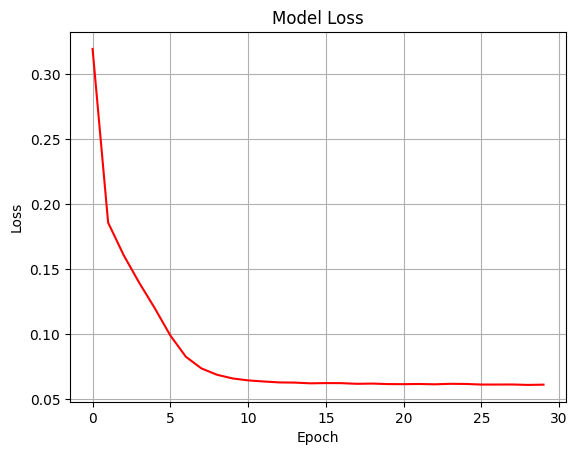
\includegraphics[width=0.78\textwidth]{ann_ldpc_training_loss.png}
\caption{Training loss of the compact ANN check-node model.}
\label{fig:ann_ldpc_training_loss}
\end{figure}

Two label scenarios are considered. In the first scenario, the ANN learns to approximate the standard SPA update. The purpose is to reproduce the mathematical behavior of SPA without computing its expensive nonlinear functions during inference. This scenario validates whether the MLP has enough capacity to learn the local update rule.

In the second scenario, the labels are modified using reliability information. If the sign of a noisy SPA message disagrees with a reference message, the label magnitude is reduced. This teaches the network not to trust a message that appears unreliable. The idea is closely related to damping and reliability control, but it is learned from data rather than manually tuned.

\begin{equation}
\mathcal{L}_{\mathrm{MAE}}=\frac{1}{N}\sum_{n=1}^{N}\left|\hat{r}_n-r_n\right|.
\end{equation}
Equation (3.14) is the MAE loss used for training. The target $r_n$ may be the SPA message or the enhanced reliability-aware label. MAE is appropriate because the objective is to approximate message values rather than classify codewords directly.

\begin{equation}
r_n=\begin{cases}r_n^{\mathrm{SPA}},&\mathrm{SPA\ label},\\ \eta_n r_n^{\mathrm{SPA}},&\mathrm{reliability\ aware\ label}.\end{cases}
\end{equation}
Equation (3.15) summarizes the two label strategies. The first case trains the ANN to imitate SPA. In the second case, $\eta_n\in[0,1]$ is a reliability factor selected during offline label construction. The reference message used to decide whether a candidate SPA message is suspicious is not an additional online input to the deployed ANN; the deployed model receives only the local vector $\mathbf{q}$ and produces the CN-to-VN update. If the reference is produced using clean transmitted bits or other information unavailable at a real receiver, the label should be interpreted as a genie-aided feasibility target for studying message attenuation, not as a deployable decoder input. Under this interpretation, the second case reduces the magnitude of unreliable messages and allows the ANN to learn a damping-like behavior that may reduce short-cycle error amplification.

\begin{equation}
\theta^{\star}=\arg\min_{\theta}\mathbb{E}_{\mathbf{q},\mathbf{r}}\left[\ell(f_{\theta}(\mathbf{q}),\mathbf{r})\right].
\end{equation}
Equation (3.16) states the training problem in expectation form. The neural function $f_\theta$ is optimized to approximate the selected target update.

\begin{equation}
\theta_{t+1}=\theta_t-\gamma_t\nabla_{\theta}\mathcal{L}(\theta_t).
\end{equation}
Equation (3.17) is the generic gradient-based parameter update. In the implementation, Adam is used instead of plain gradient descent, but the equation explains the learning principle.

\begin{equation}
\mathrm{SNR}_{\mathrm{dB}}=10\log_{10}\frac{E_s}{N_0}.
\end{equation}
Equation (3.18) denotes the SNR variable used when generating AWGN training data across multiple channel conditions.

\section{Result Interpretation and Implementation Discussion}
\subsection{Interpretation of the Two Scenarios}
The SPA-approximation scenario is conservative. It asks the ANN to behave like a known algorithm. If the ANN output is close to SPA and the BER curve is close to SPA, the model has successfully learned the nonlinear update. The value of this scenario lies in complexity reduction and hardware feasibility rather than in creating a new decoding principle.

The enhanced-label scenario is more ambitious. It does not simply imitate SPA. It uses additional knowledge to reduce the magnitude of messages suspected to be wrong. This is relevant because iterative decoding can amplify incorrect information. A wrong message with a large magnitude can be more detrimental than a weak message because it can dominate later VN decisions.

Short cycles in the Tanner graph make this issue more severe. Belief propagation assumes that incoming messages are approximately independent. Short cycles violate this assumption because information can return to a node through a short path. The ANN does not remove the short cycle, but it can learn to reduce overconfident messages that arise from correlated information.

\subsection{Performance Discussion}
The BER comparison in Figure~\ref{fig:ann_ldpc_ber_comparison} shows that the ANN approximation can achieve BER performance close to SPA and better than Min-Sum in the waterfall region of the evaluated QC-LDPC code. This is a relevant outcome because it suggests that a compact neural model can preserve the main behavior of the nonlinear CN update. The result supports the interpretation that the network is learning a structured mathematical mapping rather than an arbitrary input-output association.

\begin{figure}[H]
\centering
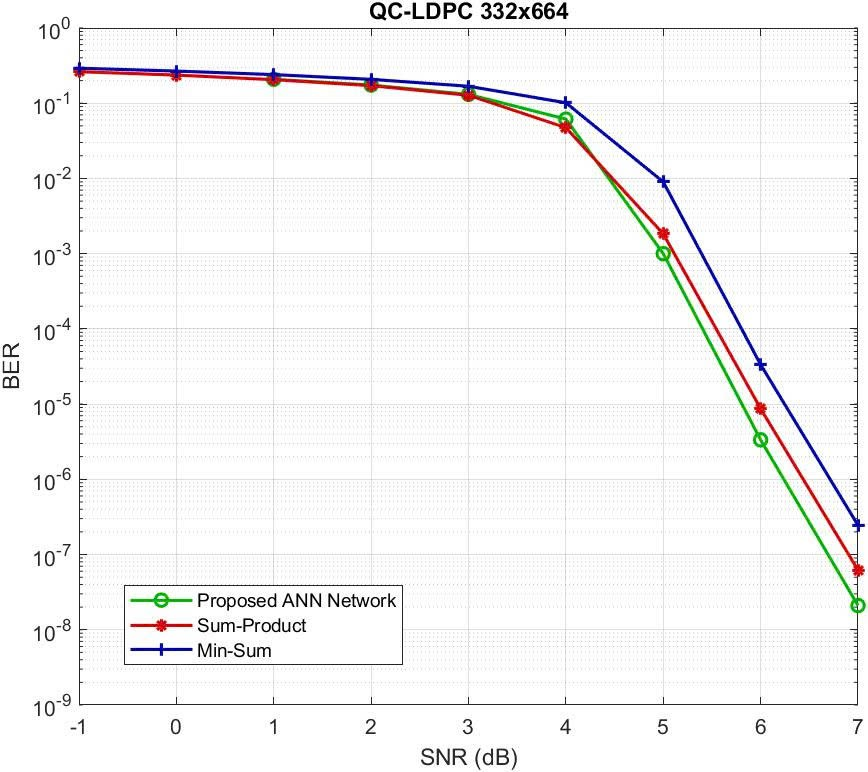
\includegraphics[width=0.86\textwidth]{ann_ldpc_ber_comparison.png}
\caption{BER comparison for QC-LDPC decoding algorithms.}
\label{fig:ann_ldpc_ber_comparison}
\end{figure}

In the enhanced-label scenario, Figure~\ref{fig:ann_ldpc_ber_comparison} indicates an approximate horizontal gain on the order of $0.2$--$0.4$ dB compared with SPA around the low-BER part of the waterfall region, especially near the $10^{-5}$ BER decade. This gain is measured under the defined QC-LDPC $(332,664)$ code, BPSK/AWGN channel, fixed training procedure, and the evaluated iteration setting. Since the current result figure does not include a complete per-SNR error-count log, the gain should be treated as a trend-level result rather than a standard-level low-BER claim. However, it provides evidence that a learned update rule can sometimes outperform the exact SPA rule when the graph contains adverse message dependencies or benefits from a reliability-aware control mechanism.

The training-loss curve supports the feasibility of the model. The loss decreases quickly in the early epochs and then stabilizes. This behavior indicates that the network learns the main nonlinear relation without excessive instability. The use of multiple SNR values in training is also important because it reduces over-specialization to a narrow reliability condition.

\begin{table}[H]
\centering
\caption{Decoder operations and interpretation for the ANN-LDPC study.}
\label{tab:ann_ldpc_decoder_comparison}
\begin{tabularx}{\textwidth}{p{0.23\textwidth}p{0.25\textwidth}Y}
\toprule
Decoder & Main operation & Interpretation in this thesis\\
\midrule
SPA & $\tanh(\cdot)$ and $\tanh^{-1}(\cdot)$ CN update & Accuracy-oriented baseline with high nonlinear-operation cost\\
Min-Sum & Sign product and minimum magnitude & Low-complexity baseline with visible BER degradation in Figure~\ref{fig:ann_ldpc_ber_comparison}\\
NMS/OMS & Fixed scaling or offset correction & Standard low-complexity references discussed analytically; not included as plotted numerical baselines in Figure~\ref{fig:ann_ldpc_ber_comparison} unless a separately tuned curve is provided\\
ANN update & Compact MLP with 49 parameters in the representative setting & Local approximation/correction of the CN update; useful when SPA-like behavior is desired without explicit transcendental functions\\
\bottomrule
\end{tabularx}
\end{table}

\subsection{Complexity and Hardware Viewpoint}
The main complexity advantage of the ANN method is the removal of explicit tanh and logarithmic operations from the SPA check-node update. In hardware, these functions usually require lookup tables, CORDIC iterations, polynomial approximations, or other special units. A compact MLP replaces these operations with multiply-add computations and ReLU activations, which are easier to pipeline and quantize.

The result should be interpreted through both BER and implementation complexity. In a practical LDPC decoder, preserving SPA-like performance while reducing the cost of nonlinear check-node computation is already meaningful. Therefore, the ANN check-node approximation offers a complexity-oriented design option, while the reliability-aware label strategy may provide additional performance improvement under selected graph, channel, and training conditions.

A fair comparison must include throughput, memory, quantization, and schedule compatibility. If ANN weights are shared across check nodes with the same degree, memory cost remains small. If the network is quantized, multipliers can be simplified. If the original LDPC schedule is retained, the method can be evaluated as a local replacement of the check-node function rather than as a fully neural decoder.

The main technical risk is generalization. A network trained for one node degree, one parity-check matrix, or one quantization format may not directly transfer to another decoder configuration. This is why the thesis treats the ANN as a model-driven approximation whose value must be assessed together with code structure, SNR range, and implementation constraints.

\subsection{Reliability-Aware Labeling and Short-Cycle Mitigation}
The enhanced-label strategy in ANN-assisted LDPC decoding deserves special attention because it is more than a numerical trick. In conventional supervised learning, the target label is often treated as ground truth. Here, however, the SPA message itself may be unreliable under noisy conditions and short-cycle effects. The training process therefore uses an adjusted label to teach the network a more cautious update behavior.

A short cycle in a Tanner graph causes information to return to a node after only a few message-passing steps. This violates the independence assumption behind belief propagation. When messages are correlated, SPA can become overconfident. In practical decoders, damping is sometimes used to reduce this problem. The proposed ANN method can be interpreted as a learned local damping mechanism whose strength depends on message~consistency.

The sign of an LLR message carries hard-decision direction, while the magnitude carries confidence. A wrong sign with small magnitude may be corrected in later iterations. A wrong sign with large magnitude can be more problematic because it suppresses contradictory information. The enhanced-label method reduces the magnitude of suspicious messages, which can reduce early convergence toward an incorrect decoder decision.

This mechanism explains why the enhanced ANN may show a favorable shift relative to SPA in the evaluated finite-length scenario. SPA is optimal on a cycle-free graph under correct probabilistic assumptions, but finite LDPC graphs contain cycles. If the graph structure and noise realization produce misleading messages, a learned damping behavior can improve practical performance. This does not contradict SPA theory; it reflects the difference between ideal assumptions and finite loopy graphs.

The method also has a connection to normalized Min-Sum. Normalized Min-Sum reduces message magnitude using a fixed factor. The enhanced ANN can be viewed as a nonlinear and data-dependent normalization. Instead of applying the same scaling everywhere, it learns when a message should be preserved and when it should be weakened. This is a more flexible form of approximation, but it requires training data and validation.

For future work, the reliability-aware label design could be extended. The reduction factor may depend on SNR, iteration index, node degree, or the distribution of incoming magnitudes. A network could also output both a message value and a confidence estimate. Such extensions would make the ANN decoder more adaptive, but they would also increase training complexity and require careful generalization tests.

The enhanced-label ANN is therefore treated as a bounded contribution. It addresses a known limitation of loopy belief propagation, while the observed gain remains dependent on label construction and on the similarity between training and test conditions.

An important engineering advantage is that the method can be introduced locally. Existing LDPC decoding schedules can be retained. Only the CN update function changes. This reduces implementation risk and makes it easier to compare the proposed method with SPA, Min-Sum, and normalized Min-Sum under identical simulation conditions.

\section{Detailed Validation and Scientific Boundaries}
\subsection{From SPA to Neural Check-Node Approximation}
The LDPC part of the thesis is strongest when it is interpreted as a model-driven neural approximation rather than a generic black-box application of deep learning. The Tanner graph already provides a precise computational structure. Each variable node represents a coded bit, each check node represents a parity constraint, and each edge carries a soft message. The neural network is introduced only at the check-node update, which is both nonlinear and repeatedly evaluated. This local formulation is important because it preserves the LDPC code constraints and avoids replacing the entire decoder by an opaque classifier.

For a parity check involving the set of variable nodes $\mathcal{N}(i)$, the constraint is
\begin{equation}
  \bigoplus_{j\in\mathcal{N}(i)} c_j=0.
\end{equation}
In belief propagation, the message from check node $i$ to variable node $j$ depends on all incoming messages from the other variable nodes connected to the same check:
\begin{equation}
  L_{i\rightarrow j}=F_{\mathrm{CN}}\left(\{L_{j'\rightarrow i}:j'\in\mathcal{N}(i)\setminus j\}\right).
\end{equation}
The exact SPA function in the LLR domain is
\begin{equation}
  F_{\mathrm{CN}}(\mathbf{q})=
  2\tanh^{-1}\left(\prod_{\ell}\tanh\frac{q_\ell}{2}\right).
\end{equation}
This function has a clear probabilistic meaning. It combines the signs of incoming messages to determine parity consistency and combines their magnitudes to determine reliability. The sign part is simple:
\begin{equation}
  \mathrm{sign}\left(F_{\mathrm{CN}}(\mathbf{q})\right)
  =
  \prod_{\ell}\mathrm{sign}(q_\ell).
\end{equation}
The difficult part is the magnitude. The magnitude depends on all incoming reliabilities through nonlinear hyperbolic functions. The Min-Sum approximation keeps only the weakest reliability:
\begin{equation}
  |F_{\mathrm{MS}}(\mathbf{q})|=\min_{\ell}|q_\ell|.
\end{equation}
This approximation is computationally efficient but systematically overestimates the SPA magnitude in many cases. Normalized Min-Sum and Offset Min-Sum correct this tendency by applying either a scaling factor or a magnitude offset. The ANN approach generalizes this idea. Instead of using one fixed correction rule, the neural network learns a nonlinear mapping from the vector of incoming magnitudes to the target output magnitude.

The check-node update can also be written through the box-plus operator:
\begin{equation}
  a\boxplus b
  =
  2\tanh^{-1}\left(\tanh\frac{a}{2}\tanh\frac{b}{2}\right).
\end{equation}
Using the Jacobian logarithm, this operation has the equivalent form
\begin{equation}
  a\boxplus b
  =
  \mathrm{sign}(ab)\min(|a|,|b|)
  +\log\left(1+e^{-|a+b|}\right)
  -\log\left(1+e^{-|a-b|}\right).
\end{equation}
The first term is the Min-Sum part. The two logarithmic terms are correction factors. This equation explains why Min-Sum works reasonably well and also why it is not exact. It also provides a theoretical interpretation of the neural model: the MLP can be seen as learning a data-dependent correction to the Min-Sum magnitude without explicitly computing the logarithmic terms.

For a check node of degree $d_c$, the input to the ANN for one outgoing edge has dimension $d_c-1$. If the decoder uses the raw incoming messages
\begin{equation}
  \mathbf{q}_{i,j}^{(t)}
  =
  [L_{j_1\rightarrow i}^{(t)},\ldots,L_{j_{d_c-1}\rightarrow i}^{(t)}]^T,
\end{equation}
then the neural approximation is
\begin{equation}
  \hat{L}_{i\rightarrow j}^{(t)}
  =
  f_\theta(\mathbf{q}_{i,j}^{(t)}).
\end{equation}
For the compact 49-parameter configuration emphasized in the reported decoder experiment, this corresponds to a degree-five local update, so $d_c-1=4$ and $\mathbf{q}_{i,j}^{(t)}\in\mathbb{R}^4$. The model should therefore not be described as a universal fixed-size replacement for arbitrary LDPC check nodes. For other degrees, the implementation must either train degree-specific networks, use a clearly defined padding or feature-selection rule, or adopt a permutation-invariant architecture.
However, the check-node function has useful symmetries. The output sign is determined by the product of input signs, while the magnitude is determined by the input magnitudes. Therefore, a more structured implementation can compute
\begin{equation}
  \hat{L}_{i\rightarrow j}^{(t)}
  =
  \left(\prod_{\ell}\mathrm{sign}(q_\ell)\right)
  g_\theta(|q_1|,\ldots,|q_{d_c-1}|).
\end{equation}
This structure reduces the burden on the neural network because the network does not need to learn sign symmetry from data. It only learns the magnitude correction. Even when a compact MLP is used directly for the update function, this symmetry-based interpretation is important for later hardware-oriented design refinement.

\subsection{Training Data, Label Design, and Validation Logic}
The quality of an ANN-assisted decoder depends strongly on how training labels are constructed. In the SPA-approximation scenario, the target label is the exact or high-precision SPA check-node output:
\begin{equation}
  r^{\mathrm{target}}=F_{\mathrm{SPA}}(\mathbf{q}).
\end{equation}
This scenario tests whether the MLP can learn a deterministic nonlinear function. If the network approximates SPA accurately over the message range used during decoding, the expected BER should be close to SPA. The benefit is then complexity reduction, especially if the neural function is easier to quantize or pipeline than the original nonlinear function.

In the reliability-aware scenario, the target is modified:
\begin{equation}
  r^{\mathrm{target}}=\rho(\mathbf{q},s,\mathrm{SNR})F_{\mathrm{SPA}}(\mathbf{q}),
\end{equation}
where $\rho$ is a reliability factor. In a simple form, $\rho<1$ when a message is suspected to be unreliable and $\rho\approx 1$ otherwise. This strategy is related to the following damping rule:
\begin{equation}
  L^{(t)}_{\mathrm{damped}}
  =
  \delta L^{(t)}+(1-\delta)L^{(t-1)},
\end{equation}
but it is more flexible because the attenuation can depend on the local message pattern rather than on a fixed global scalar.

The label design must be treated carefully. If the reliability-aware label is generated using information that would not be available in a real decoder, then the trained model may implicitly learn from an unrealistic oracle. This does not invalidate the study, but it changes the interpretation. The result should be described as evidence that message-magnitude control can improve finite-length loopy decoding under selected conditions, not as a universal guarantee of superiority over SPA. This is why the thesis uses restrained language when discussing the approximate $0.2$--$0.4$ dB trend-level gain observed in Figure~\ref{fig:ann_ldpc_ber_comparison}.

The same distinction applies to reference messages used during label construction. A reference message can be generated offline from a cleaner SPA computation, a known transmitted codeword, or another teacher rule. Such information is used only to construct targets for training. During inference, the deployed ANN receives the local incoming-message vector $\mathbf{q}_{i,j}^{(t)}$ and does not receive the transmitted bits, a clean-channel message, or an explicit oracle flag. If the target construction uses information unavailable online, the result should be interpreted as a feasibility study of learned damping and reliability control.

A robust validation procedure should separate training, validation, and testing SNR ranges. If training uses only one SNR, the network may learn a narrow message distribution. For example, at high SNR most LLR magnitudes are large and signs are reliable; at low SNR magnitudes are small and sign errors are frequent. A neural correction trained only at high SNR may overtrust messages at low SNR. A neural correction trained only at low SNR may unnecessarily damp messages at high SNR. Therefore, training over a range of SNR values is more appropriate for a decoder intended to operate across channel conditions.

Let $\mathcal{S}_{\mathrm{train}}$ be the set of SNR values used in training and $\mathcal{S}_{\mathrm{test}}$ be the set used in testing. The most informative evaluation includes both interpolation and extrapolation:
\begin{equation}
  \mathcal{S}_{\mathrm{test}}
  =
  \mathcal{S}_{\mathrm{interp}}\cup\mathcal{S}_{\mathrm{extra}},
\end{equation}
where $\mathcal{S}_{\mathrm{interp}}$ lies inside the training range and $\mathcal{S}_{\mathrm{extra}}$ lies outside it. A model that works only in interpolation may still be useful, but the operating range must be stated clearly.

The loss function also affects the learned behavior. MAE penalizes absolute message error:
\begin{equation}
  \mathcal{L}_{\mathrm{MAE}}=\frac{1}{N}\sum_{n=1}^{N}|\hat{r}_n-r_n|.
\end{equation}
Mean-square error would penalize large errors more strongly:
\begin{equation}
  \mathcal{L}_{\mathrm{MSE}}=\frac{1}{N}\sum_{n=1}^{N}(\hat{r}_n-r_n)^2.
\end{equation}
For LLR messages, the best loss is not always obvious. A small absolute error near zero can change the hard decision sign and may be more harmful than a larger magnitude error when the sign is already reliable. A sign-aware loss could include an additional penalty:
\begin{equation}
  \mathcal{L}_{\mathrm{sign}}
  =
  \mathcal{L}_{\mathrm{MAE}}
  +
  \lambda
  \frac{1}{N}\sum_{n=1}^{N}
  \mathbf{1}\{\mathrm{sign}(\hat{r}_n)\ne\mathrm{sign}(r_n)\}.
\end{equation}
This thesis does not require such a loss to justify the current results, but discussing it clarifies the connection between regression accuracy and decoding~performance.

\subsection{Complexity Accounting for ANN-Assisted LDPC Decoding}
A precise complexity assessment requires more than the statement that the neural network is small. The number of parameters is one part of the argument, but the number of operations per iteration and the memory-access pattern are also important. Consider a one-hidden-layer MLP with input dimension $d_{\mathrm{in}}$, hidden dimension $d_h$, and output dimension $d_{\mathrm{out}}=1$. The number of weights and biases is
\begin{equation}
  N_\theta=d_{\mathrm{in}}d_h+d_h+d_h d_{\mathrm{out}}+d_{\mathrm{out}},
\end{equation}
where the first two terms belong to the hidden layer and the last two terms belong to the output layer. The number of multiply-accumulate operations per inference is approximately
\begin{equation}
  C_{\mathrm{MLP}}\approx d_{\mathrm{in}}d_h+d_h d_{\mathrm{out}}.
\end{equation}
For the representative 49-parameter configuration used in this thesis, $d_{\mathrm{in}}=4$, $d_h=8$, and $d_{\mathrm{out}}=1$. The inference cost is therefore about $4\times 8+8\times 1=40$ multiply-accumulate operations per outgoing message, plus ReLU comparisons. Whether this is cheaper than SPA depends on the hardware cost assigned to tanh, inverse tanh, or lookup-table access. In digital hardware, a multiply-add may be cheaper and easier to pipeline than a high-precision transcendental operation, especially when weights are quantized.

If a Tanner graph has $E$ edges and the decoder runs $I_{\max}$ iterations, a local check-node update is evaluated on the order of $E I_{\max}$ times. The total ANN operation count is therefore approximately
\begin{equation}
  C_{\mathrm{total}}\approx E I_{\max} C_{\mathrm{MLP}}.
\end{equation}
This expression shows why the network must remain compact. A large neural network may look acceptable for one check-node update, but the cost is multiplied by all edges and all iterations. The local MLP architecture is therefore a more defensible design than a large end-to-end decoder.

Memory cost also matters. If one set of weights is shared across all check nodes of the same degree, the parameter memory is small:
\begin{equation}
  M_{\theta}=N_{\theta}Q_w,
\end{equation}
where $Q_w$ is the number of bits per weight. With 8-bit quantization and 49 parameters, the weight memory is only a few hundred bits. If separate weights were learned for each node or each iteration, the memory cost would increase substantially. The thesis therefore favors weight sharing and model-driven structure because they are consistent with a practical receiver.

Quantization can be incorporated into the neural model. A fixed-point network computes
\begin{equation}
  \hat{r}=Q_o\left(f_{Q_\theta(\theta)}(Q_i(\mathbf{q}))\right),
\end{equation}
where $Q_i$, $Q_\theta$, and $Q_o$ are quantizers for input messages, weights, and output messages. Quantization-aware training can simulate these quantizers during training so that the network learns parameters robust to finite precision. This would be an important continuation of the current work because LDPC decoders are usually implemented with fixed-point messages.

\subsection{Scientific Interpretation of the Observed Gains}
The gain of the enhanced ANN scenario should be presented as a conditional result. In communication research, a BER improvement is meaningful only when the code, block length, modulation, channel model, decoder schedule, iteration count, and simulation length are known. A curve obtained for one QC-LDPC code over AWGN cannot be generalized to all LDPC codes or all BIBCM-ID configurations. The thesis therefore interprets the gain as evidence that learned reliability control can improve a specific finite-length loopy decoder.

This interpretation is scientifically stronger than an exaggerated claim. SPA is optimal for tree-like factor graphs under correct probability models, but practical LDPC graphs contain cycles. In a loopy graph, messages can become correlated. When correlated messages are repeatedly combined, the decoder may become overconfident. Reliability-aware attenuation can reduce this effect. The ANN method is thus not contradicting the theory of SPA; it is exploiting the difference between the ideal assumptions behind SPA and the finite-length conditions of practical decoding.

The decoder-side result is also relevant to BIBCM-ID because the Demodulation block may deliver imperfect LLRs. If the Demodulation output is slightly biased or overconfident, a reliability-aware LDPC update may prevent the decoder from amplifying that bias too quickly. This is a plausible system-level benefit even before joint optimization of Modulation and decoding is considered. The ANN decoder is therefore treated as a controlled modification inside the channel decoder, while AutoEncoder Modulation is treated as a complementary investigation of the soft-information source.

The complexity benefit depends on the implementation baseline. Compared with Min-Sum, the ANN may be more complex. Compared with exact SPA using tanh and inverse tanh, the ANN may be more hardware-friendly. Therefore, the fair statement is not that the ANN is always the lowest-complexity decoder, but that it offers a trade-off between SPA-like performance and implementable nonlinear approximation.

Generalization remains an engineering requirement and can be tested through multiple parity-check matrices, multiple node degrees, multiple SNR ranges, quantized messages, and mismatched channel conditions. This does not weaken the current contribution; it places it at the correct level of evidence. The study demonstrates a focused method and interprets it with appropriate technical~boundaries.

\section{Evaluation Protocol for ANN-Assisted Decoding}
A technically convincing decoder study requires an evaluation protocol that separates algorithmic effect from simulation artifact. The BER curve is the most visible result, but it is not the only evidence. A fair comparison requires the baseline algorithms to use the same code, modulation, channel model, iteration limit, stopping rule, and LLR scaling. If any of these conditions differ, the comparison may reflect an implementation difference rather than a true decoding advantage.

The first requirement is a consistent code configuration. For an LDPC code with block length $n$, information length $k$, and rate $R_c=k/n$, every compared decoder should operate on the same parity-check matrix $\mathbf{H}$. If the ANN is trained for a QC-LDPC matrix, the test should clearly state whether the same matrix is used or whether a different matrix is used for generalization. A decoder that performs well on one structured matrix may not automatically transfer to another because the distribution of node degrees, short cycles, and trapping sets changes.

The second requirement is a consistent channel and modulation setting. If the training data are generated from BPSK over AWGN, then the first validation should use the same setting to isolate the check-node approximation. Only after that should the method be tested with higher-order Modulation or with BIBCM-ID-style soft Demodulation input. This staged evaluation is important. It prevents a single experiment from mixing too many effects: channel mismatch, Demodulation mismatch, LDPC graph behavior, and neural approximation error.

The third requirement is a sufficient number of simulated bits. At low BER, a small number of errors produces a noisy estimate. If $N_{\mathrm{err}}$ errors are observed over $N_{\mathrm{bit}}$ transmitted bits, the BER estimate is
\begin{equation}
  \widehat{\mathrm{BER}}=\frac{N_{\mathrm{err}}}{N_{\mathrm{bit}}}.
\end{equation}
For rare errors, the relative uncertainty is large when $N_{\mathrm{err}}$ is small. A simple rule in communication simulations is to collect a minimum number of error events before trusting a point on a BER curve. Therefore, a low-BER point based on too few errors is interpreted only as an indicative trend rather than as strong evidence of superiority.

The fourth requirement is to report the iteration limit and stopping rule. A syndrome-based stopping rule terminates decoding when
\begin{equation}
  \mathbf{H}\hat{\mathbf{c}}^T=\mathbf{0}.
\end{equation}
For the ANN-LDPC result, the comparison is interpreted as a same-protocol evaluation, but the extracted material does not provide a complete per-SNR record of $I_{\max}$, stopping-rule status, and average iteration count. These quantities must be included in the final simulation archive before making strong implementation-level claims. If one decoder reaches the syndrome condition earlier than another, it may reduce average complexity even when the maximum iteration limit is the same. Therefore, average iteration count is a useful companion metric:
\begin{equation}
  \bar{I}=\frac{1}{N_f}\sum_{r=1}^{N_f}I_r,
\end{equation}
where $N_f$ is the number of simulated frames and $I_r$ is the number of iterations used for frame $r$. A decoder that preserves BER while reducing $\bar{I}$ can be attractive even if its per-iteration cost is slightly higher.

The fifth requirement is to include frame error rate when possible. BER measures the fraction of wrong bits, while FER measures whether the entire frame is decoded correctly:
\begin{equation}
  \mathrm{FER}=\frac{N_{\mathrm{frame,err}}}{N_{\mathrm{frame}}}.
\end{equation}
In coded systems, FER is often important because many applications treat a frame with one error as unusable. An ANN check-node update that reduces BER but leaves FER unchanged may still be useful, but the distinction should be understood.

\section{Ablation View of the ANN Decoder}
An ablation view clarifies which part of the method is responsible for the observed behavior. The first ablation is SPA imitation versus reliability-aware labeling. If the SPA-imitation network matches SPA, this supports the claim that the MLP can approximate the nonlinear check-node function. If the reliability-aware network improves the curve, this supports the additional claim that learned magnitude control can be beneficial under finite loopy decoding. These two claims should be evaluated separately.

The second ablation is network size. A compact network is central to the engineering argument. If a larger network improves BER slightly but greatly increases cost, it may be less relevant to a receiver implementation. Therefore, the hidden-layer size should be interpreted as a design variable in the performance-complexity trade-off:
\begin{equation}
  \mathrm{Tradeoff}=
  \left(\mathrm{BER},\ \mathrm{FER},\ \bar{I},\ C_{\mathrm{op}},\ M_{\theta}\right),
\end{equation}
where $C_{\mathrm{op}}$ denotes computational operations and $M_{\theta}$ denotes model memory. This vector view is more informative than a single BER number.

The third ablation is message clipping. LDPC decoders often clip LLRs to a finite range. If the ANN is trained on unclipped floating-point SPA messages but tested in a clipped decoder, performance may change. A fair test should either train and test under the same clipping range or explicitly analyze the mismatch. The clipping range can be written as
\begin{equation}
  L_{\mathrm{clip}}=\max(-L_{\max},\min(L,L_{\max})).
\end{equation}
The value of $L_{\max}$ affects both numerical stability and decoding confidence.

The fourth ablation is node degree. A single MLP may be trained for one check-node degree. If the LDPC matrix has multiple check-node degrees, the decoder can either use separate networks for each degree, pad inputs to a common dimension, or design a permutation-invariant architecture. Separate networks increase memory. Padding may waste computation. A permutation-invariant architecture can be written as
\begin{equation}
  g_\theta(\{|q_\ell|\})=
  \rho_\theta\left(\sum_{\ell}\psi_\theta(|q_\ell|)\right),
\end{equation}
where $\psi_\theta$ and $\rho_\theta$ are learnable functions. This form respects the fact that the check-node update should not depend on the arbitrary order in which messages are listed.

The fifth ablation is iteration dependence. A network can share the same parameters across all iterations or use iteration-specific parameters. Shared parameters reduce memory and are easier to justify. Iteration-specific parameters may improve performance but risk overfitting to a fixed iteration schedule. For a practical decoder, shared or lightly parameterized iteration dependence is preferable unless the gain is substantial.

\section{Scientific Boundaries of the Decoder Study}
The comparison between the ANN decoder and normalized Min-Sum should be interpreted through both performance and implementation criteria. Normalized Min-Sum is extremely simple and may be preferable when minimum complexity is the only goal. The ANN method is more relevant when the designer wants SPA-like behavior without explicit transcendental functions, or when reliability-aware damping provides a controlled advantage. The result is therefore a trade-off, not a universal replacement.

The statistical reliability of a BER gain depends on simulation length and the number of observed errors. Figure~\ref{fig:ann_ldpc_ber_comparison} shows a favorable trend under the stated QC-LDPC and BPSK/AWGN conditions, while standard-level claims in lower-BER regions would require longer simulations and explicit error-event logging at each SNR point. This interpretation is consistent with a study centered on algorithmic analysis and feasibility assessment.

A complete reproduction table should include, for each SNR point, the number of transmitted frames, the number of transmitted information bits, the number of observed bit errors, the number of frame errors, and the stopping outcome if early termination is enabled. Without these fields, the BER curve remains useful for comparing trends among algorithms, but its low-BER tail should not be overinterpreted.

The ANN does not remove the interpretability of LDPC decoding because the proposed method preserves the Tanner graph and changes only a local update function. The parity-check matrix, syndrome test, variable-node update, and iterative schedule remain interpretable. The MLP acts as a learned approximation or correction for the nonlinear check-node operation. This is very different from replacing the decoder by a neural classifier that directly maps channel samples to messages.

The method is compatible with soft information from BIBCM-ID Demodulation at the message-interface level: the LDPC decoder consumes LLRs regardless of whether they originate from BPSK Demodulation or high-order BIBCM-ID Demodulation. However, the distribution of those LLRs may differ. BPSK-AWGN is therefore a controlled first evaluation, while BIBCM-ID soft input is the broader system context.

These possible challenges are not defects if they are addressed explicitly. They define the boundary between a focused master's-level contribution and a full standard-ready receiver implementation. The thesis uses this boundary to keep the claims credible: ANN-assisted check-node processing is the central contribution; AutoEncoder Modulation is a supporting analysis of the soft-information source; broader multi-channel validation remains an engineering continuation.


\section{Chapter Conclusion}
This chapter has analyzed ANN-assisted LDPC decoding as the main technical contribution of the thesis. Starting from the Tanner-graph representation and the LLR-domain message-passing equations, the chapter identified the check-node update as a computationally demanding part of SPA decoding. The Min-Sum approximation reduces this cost but loses part of the nonlinear correction present in SPA. This trade-off motivates the use of a compact neural model as a local approximation or correction of the check-node operation.

The proposed neural direction is deliberately model-driven. The parity-check matrix, variable-node update, syndrome test, and iterative decoding schedule remain unchanged; only the local check-node update is approximated or adjusted. In the representative configuration, the MLP uses four input reliability values, eight hidden units, and one output value, giving 49 trainable parameters and about 40 multiply-accumulate operations per outgoing message. This compact scale is essential for a decoder block that is evaluated many times over all Tanner-graph edges and decoding iterations.

The BER results support two conclusions with different levels of claim. First, the ANN trained to imitate SPA can preserve decoding behavior close to SPA while avoiding explicit tanh and inverse-tanh computations. This result is mainly a complexity-oriented contribution. Second, the reliability-aware label strategy shows that learned message attenuation can improve practical decoding behavior in the evaluated finite-length loopy graph. This gain is interpreted conditionally rather than universally, because it depends on the code, channel model, training labels, SNR range, and simulation length. The chapter therefore positions ANN-assisted LDPC decoding as a practical hybrid method: it keeps the structure of classical coding theory while using learning to approximate or regulate a nonlinear message update.

\chapter*{CONCLUSION AND RECOMMENDATIONS}
\addcontentsline{toc}{chapter}{\textbf{CONCLUSION AND RECOMMENDATIONS}}
This thesis has studied the utilization of artificial neural networks in LDPC decoding for BIBCM-ID-oriented communication systems. The theoretical part reviewed the role of Modulation, Demodulation, interleaving, soft information, channel decoding, and model-driven deep learning in iterative coded modulation. This foundation clarifies why the quality of LLR messages is a central issue: the LDPC decoder operates on reliability information, and incorrect or overconfident messages can reduce iterative-decoding effectiveness.

\noindent\textbf{Validated decoder result.} The main technical contribution is the analysis of ANN-assisted LDPC decoding. A compact neural model is used to approximate the check-node update, which is one of the nonlinear and computationally expensive operations in SPA decoding. In the representative configuration, the MLP uses four input values, eight hidden units, one output value, and 49 trainable parameters; the corresponding inference cost is about 40 multiply-accumulate operations per outgoing message plus ReLU comparisons. For the QC-LDPC $(332,664)$ code over the BPSK/AWGN channel, Figure~\ref{fig:ann_ldpc_ber_comparison} shows that the ANN update follows the SPA curve closely and improves over Min-Sum in the waterfall region under the plotted conditions. In the enhanced-label case, the plotted curve indicates an approximate $0.2$--$0.4$ dB horizontal shift around the $10^{-5}$ BER decade. These results should be interpreted primarily in terms of complexity reduction, preservation of SPA-like decoding quality, and reliability-aware message control under the stated simulation conditions.

\noindent\textbf{Supporting system analysis.} The AutoEncoder Modulation study is included as a complementary analysis of the Modulation and Demodulation side of the BIBCM-ID soft-information chain. The simulation results in Chapter 2 show that learned signal representations can adapt to PA distortion, CFO, fading, and sequence-dependent channel effects. This part strengthens the discussion of how upstream signal mapping and receiver observation quality affect LDPC decoding, while the main quantitative evidence for the thesis remains the ANN-LDPC decoder analysis presented in Chapter 3.

\noindent\textbf{Recommendations.} Overall, the thesis supports a hybrid view of deep learning in communication systems. Neural networks are most defensible when they approximate difficult nonlinear operations, correct model mismatch, or improve the reliability of soft information while preserving the structure of established coding and modulation theory. Future work should focus on calibrated bit-level LLR output for neural Demodulation, broader validation over LDPC code structures and channel conditions, fixed-point and quantization-aware ANN decoder design, and complexity-throughput evaluation for practical receiver architectures. For the ANN-LDPC result specifically, a final simulation package should include the parity-check matrix, $I_{\max}$, stopping rule, random seeds, and per-SNR frame/error logs so that the reported BER trends can be reproduced and, where sufficient error counts are available, promoted to stronger statistical claims.
\begin{thebibliography}{99}
\addcontentsline{toc}{chapter}{\textbf{REFERENCES}}
\item[]\textbf{English:}
\bibitem{bishop2006} C. M. Bishop, Pattern Recognition and Machine Learning. Springer, 2006.
\bibitem{lecun2015} Y. LeCun, Y. Bengio, and G. Hinton, ``Deep learning,'' Nature, vol. 521, pp. 436--444, 2015.
\bibitem{goodfellow2016} I. Goodfellow, Y. Bengio, and A. Courville, Deep Learning. MIT Press, 2016.
\bibitem{shannon1948} C. E. Shannon, ``A mathematical theory of communication,'' Bell System Technical Journal, vol. 27, no. 3, pp. 379--423, 1948.
\bibitem{gallager1962} R. G. Gallager, ``Low-density parity-check codes,'' IRE Transactions on Information Theory, vol. 8, no. 1, pp. 21--28, 1962.
\bibitem{tanner1981} R. M. Tanner, ``A recursive approach to low complexity codes,'' IEEE Transactions on Information Theory, vol. 27, no. 5, pp. 533--547, 1981.
\bibitem{mackay1996} D. J. C. MacKay and R. M. Neal, ``Near Shannon limit performance of low density parity check codes,'' Electronics Letters, vol. 32, no. 18, pp. 1645--1646, 1996.
\bibitem{kschischang2001} F. R. Kschischang, B. J. Frey, and H.-A. Loeliger, ``Factor graphs and the sum-product algorithm,'' IEEE Transactions on Information Theory, vol. 47, no. 2, pp. 498--519, 2001.
\bibitem{richardson2008} T. Richardson and R. Urbanke, Modern Coding Theory. Cambridge University Press, 2008.
\bibitem{hu2005peg} X.-Y. Hu, E. Eleftheriou, and D. M. Arnold, ``Regular and irregular progressive edge-growth Tanner graphs,'' IEEE Transactions on Information Theory, vol. 51, no. 1, pp. 386--398, 2005.
\bibitem{hu2001spa} X.-Y. Hu, E. Eleftheriou, D. M. Arnold, and A. Dholakia, ``Efficient implementations of the sum-product algorithm for decoding LDPC codes,'' in Proc. IEEE GLOBECOM, 2001.
\bibitem{chen2002} J. Chen and M. P. C. Fossorier, ``Near optimum universal belief propagation based decoding of low-density parity-check codes,'' IEEE Transactions on Communications, vol. 50, no. 3, pp. 406--414, 2002.
\bibitem{zarkeshvari2002} F. Zarkeshvari and A. H. Banihashemi, ``On implementation of min-sum algorithm for decoding low-density parity-check codes,'' in Proc. IEEE GLOBECOM, 2002.
\bibitem{zehavi1992} E. Zehavi, ``8-PSK trellis codes for a Rayleigh channel,'' IEEE Transactions on Communications, vol. 40, no. 5, pp. 873--884, 1992.
\bibitem{caire1998} G. Caire, G. Taricco, and E. Biglieri, ``Bit-interleaved coded modulation,'' IEEE Transactions on Information Theory, vol. 44, no. 3, pp. 927--946, 1998.
\bibitem{li1997} X. Li and J. A. Ritcey, ``Bit-interleaved coded modulation with iterative decoding,'' IEEE Communications Letters, vol. 1, no. 6, pp. 169--171, 1997.
\bibitem{li1998} X. Li, A. Chindapol, and J. A. Ritcey, ``Bit-interleaved coded modulation with iterative decoding and 8PSK signaling,'' IEEE Transactions on Communications, vol. 50, no. 8, pp. 1250--1257, 2002.
\bibitem{tenbrink2001} S. ten Brink, ``Convergence behavior of iteratively decoded parallel concatenated codes,'' IEEE Transactions on Communications, vol. 49, no. 10, pp. 1727--1737, 2001.
\bibitem{brink2004} S. ten Brink, G. Kramer, and A. Ashikhmin, ``Design of low-density parity-check codes for modulation and detection,'' IEEE Transactions on Communications, vol. 52, no. 4, pp. 670--678, 2004.
\bibitem{hagenauer1996} J. Hagenauer, E. Offer, and L. Papke, ``Iterative decoding of binary block and convolutional codes,'' IEEE Transactions on Information Theory, vol. 42, no. 2, pp. 429--445, 1996.
\bibitem{nachmani2016} E. Nachmani, Y. Be'ery, and D. Burshtein, ``Learning to decode linear codes using deep learning,'' in Proc. Allerton Conference on Communication, Control, and Computing, 2016.
\bibitem{nachmani2018} E. Nachmani, E. Marciano, L. Lugosch, W. J. Gross, D. Burshtein, and Y. Be'ery, ``Deep learning methods for improved decoding of linear codes,'' IEEE Journal of Selected Topics in Signal Processing, vol. 12, no. 1, pp. 119--131, 2018.
\bibitem{lugosch2017} L. Lugosch and W. J. Gross, ``Learning from the syndrome,'' in Proc. Asilomar Conference on Signals, Systems, and Computers, 2017.
\bibitem{kuck2020} J. Kuck, S. Han, and S. Mohan, ``Belief propagation neural networks,'' Advances in Neural Information Processing Systems, vol. 33, pp. 667--678, 2020.
\bibitem{wang2022} Q. Wang, S. ten Brink, and H. V. Poor, ``Normalized min-sum neural network for LDPC decoding,'' IEEE Transactions on Cognitive Communications and Networking, vol. 9, no. 1, pp. 70--81, 2023.
\bibitem{oshea2017} T. J. O'Shea and J. Hoydis, ``An introduction to deep learning for the physical layer,'' IEEE Transactions on Cognitive Communications and Networking, vol. 3, no. 4, pp. 563--575, 2017.
\bibitem{dorner2018} S. Dorner, S. Cammerer, J. Hoydis, and S. ten Brink, ``Deep learning based communication over the air,'' IEEE Journal of Selected Topics in Signal Processing, vol. 12, no. 1, pp. 132--143, 2018.
\bibitem{aoudia2019} F. A. Aoudia and J. Hoydis, ``End-to-end learning of communications systems without a channel model,'' in Proc. Asilomar Conference on Signals, Systems, and Computers, 2018.
\bibitem{cammerer2020} S. Cammerer, F. A. Aoudia, S. Dorner, M. Stark, J. Hoydis, and S. ten Brink, ``Trainable communication systems: Concepts and prototype,'' IEEE Transactions on Communications, vol. 68, no. 9, pp. 5489--5503, 2020.
\bibitem{guo2017} C. Guo, G. Pleiss, Y. Sun, and K. Q. Weinberger, ``On calibration of modern neural networks,'' in Proc. International Conference on Machine Learning, pp. 1321--1330, 2017.
\bibitem{rapp1991} C. Rapp, ``Effects of HPA-nonlinearity on a 4-DPSK/OFDM-signal for a digital sound broadcasting system,'' in Proc. European Conference on Satellite Communications, 1991.
\bibitem{saleh1981} A. A. M. Saleh, ``Frequency-independent and frequency-dependent nonlinear models of TWT amplifiers,'' IEEE Transactions on Communications, vol. 29, no. 11, pp. 1715--1720, 1981.
\bibitem{proakis2008} J. G. Proakis and M. Salehi, Digital Communications, 5th ed. McGraw-Hill, 2008.
\bibitem{goldsmith2005} A. Goldsmith, Wireless Communications. Cambridge University Press, 2005.
\end{thebibliography}
\appendix
\chapter*{SCIENTIFIC PUBLICATIONS}
\addcontentsline{toc}{chapter}{\textbf{SCIENTIFIC PUBLICATIONS}}

\begin{enumerate}[label=\arabic*., leftmargin=1.2cm, itemsep=0.35cm]
\item Lại Tiến Đệ, Phạm Xuân Nghĩa, \textit{``Ứng dụng mạng nơ-ron nhân tạo cho giải mã LDPC nhằm tăng chất lượng và giảm độ phức tạp bộ giải mã,''} in \textit{REV-ECIT lần thứ 28}, 2025.

\item Lai Tien De, Pham Xuan Nghia, Tran Duc Trung, \textit{``Intelligent AutoEncoder-Based Modulation: Optimizing Transmission Performance over Non-Ideal Wireless Channels,''} in \textit{REV-JOURNAL}, May 2026.
\end{enumerate}

\clearpage
\chapter*{CURRICULUM VITAE}
\addcontentsline{toc}{chapter}{\textbf{CURRICULUM VITAE}}

\noindent\textbf{Full name:} Lai Tien De

\noindent\textbf{Date of birth:} \dotfill \hfill \textbf{Place of birth:} \dotfill

\noindent\textbf{Contact address:} \dotfill

\vspace{0.8cm}
\noindent\textbf{Education:}

\vspace{0.4cm}
\noindent\dotfill

\vspace{0.4cm}
\noindent\dotfill

\vspace{0.8cm}
\noindent\textbf{Working history:}

\vspace{0.4cm}
\noindent\dotfill

\vspace{0.4cm}
\noindent\dotfill

\clearpage
\chapter*{CONFIRMATION OF THESIS ELIGIBILITY FOR DEFENSE}
\addcontentsline{toc}{chapter}{\textbf{CONFIRMATION OF THESIS ELIGIBILITY FOR DEFENSE}}

\noindent\textbf{Thesis author:} Lai Tien De

\noindent\textbf{Thesis title:} Utilization of Artificial Neural Networks in LDPC Decoding for BIBCM-ID Systems

\noindent\textbf{Field:} Telecommunications Engineering

\noindent\textbf{Major:} Telecommunications Engineering

\noindent\textbf{Code:} \dotfill

\noindent\textbf{Scientific supervisors:} Dr. Pham Xuan Nghia; Dr. Hoang Van Dung

\vspace{0.5cm}
\noindent The thesis is confirmed to be eligible for defense before the Master's Thesis Evaluation Council.

\vspace{1.6cm}
\noindent\begin{tabularx}{\textwidth}{>{\centering\arraybackslash}X>{\centering\arraybackslash}X}
\textbf{SCIENTIFIC SUPERVISOR} & \textbf{THESIS AUTHOR}\\[1.8cm]
(Signature and full name) & (Signature and full name)
\end{tabularx}

\vspace{1.6cm}
\noindent\begin{tabularx}{\textwidth}{>{\centering\arraybackslash}X>{\centering\arraybackslash}X}
\textbf{DEPARTMENT/FACULTY HEAD} & \textbf{PROGRAM MANAGEMENT OFFICER}\\[1.8cm]
(Signature and full name) & (Signature and full name)
\end{tabularx}

\clearpage
\chapter*{THESIS REVISION CONFIRMATION (IF ANY)}
\addcontentsline{toc}{chapter}{\textbf{THESIS REVISION CONFIRMATION (IF ANY)}}
\enlargethispage{1.5cm}

\begin{center}
\textbf{SOCIALIST REPUBLIC OF VIETNAM}\\
\textbf{Independence -- Freedom -- Happiness}
\end{center}

\vspace{0.4cm}
\noindent\textbf{Thesis author:} Lai Tien De

\noindent\textbf{Thesis title:} Utilization of Artificial Neural Networks in LDPC Decoding for BIBCM-ID Systems

\noindent\textbf{Field:} Telecommunications Engineering

\noindent\textbf{Major:} Telecommunications Engineering

\noindent\textbf{Code:} \dotfill

\noindent\textbf{Scientific supervisors:} Dr. Pham Xuan Nghia; Dr. Hoang Van Dung

\vspace{0.25cm}
\noindent The thesis author and scientific supervisors confirm that the thesis has been revised according to the Evaluation Council meeting minutes dated \dotfill, with the following contents:

\vspace{0.25cm}
\noindent\dotfill

\vspace{0.25cm}
\noindent\dotfill

\vspace{0.25cm}
\noindent\dotfill

\vspace{0.45cm}
\noindent Date \dotfill\ Month \dotfill\ Year \dotfill

\vspace{0.55cm}
\noindent\begin{tabularx}{\textwidth}{>{\centering\arraybackslash}X>{\centering\arraybackslash}X}
\textbf{SCIENTIFIC SUPERVISOR} & \textbf{THESIS AUTHOR}\\[1.6cm]
(Signature and full name) & (Signature and full name)
\end{tabularx}

\vspace{0.65cm}
\begin{center}
\textbf{COUNCIL CHAIRPERSON OR SECRETARY}\\[1.1cm]
(Signature and full name)
\end{center}

\end{document}
